\documentclass{morningstar}

\title{基于谷歌云的在线音频修复系统设计}
\entitle{An Online Audio Restoration System \linebreak On Google Cloud Engine}
\major{电子信息工程}
\class{国电1702}
\id{1406170213}
\author{吉普}
\instructor{李义丰}
\period{2020.12～2021.6}

\begin{document}

\setfontformat
\makecover

\clearpage

\showcntitle

\sectionWithStar{摘要}

由于语音信号是一种非平稳信号，使用传统的方式处理起来比较困难。
本文利用小波多尺度分析的特点，使用最新的小波阈值去噪算法实现对语音的去噪。
为了克服现有阈值算法的缺陷，本文提出了对高频噪声处理效果良好的软硬折中阈值去噪算法，有效增强了去噪效果。

随着云技术的发展，越来越多的工具被集成到了云端，
针对这一趋势，本文设计并搭建了一个基于Django的网络应用，
并通过容器技术部署到谷歌云服务器，为用户提供音频文件的在线修复。    

\showcnkeywords{语音去噪, 时频分析, 小波阈值去噪, 网络应用}

\startfrontpart

\clearpage

\showentitle

\sectionWithStar{Abstract}

Since the speech signal is a non-stationary signal, it is difficult to process it in a traditional way.
This paper analyze speech signal with the multi-resolution analysis of wavelet and realize the denoising of speech signal with the latest wavelet threshold denoising algorithm.
In order to overcome the drawback of the existing threshold algorithm, a new threshold method which compromise between soft and hard denoising algorithm is proposed. The new threshold method has better effect on high-frequency noise processing.

With the development of cloud technology, more and more tools are integrated into the cloud,
In response to this trend, this article designed and built a Django-based web application,
which has deployed to Google Cloud Platform through container technology to provide users with online repair of audio files.

\showenkeywords{Speech Denoising, Time-frequency analysis, Wavelet Denoise, Web Development}



\clearpage
\tableofcontents



\clearpage
\startmainpart
\section{绪论}
\subsection{课题研究背景和意义}

在音频修复领域，对于专业人士，可以选用iZotope、JAMin等获取成本，学习成本都非常高的音频修复软件；
对于非专业人士，他们实际上也具有较强的短期音频修复需求，例如修复损坏的历史音频和嘈杂的课堂录音。
但苦于缺少门槛较低、随手可及的音频修复工具，被迫忍受糟糕音质带来的不便。

此外，在线音频修复平台不该只是面向普通用户，还应提供完善的技术文档与开发套件，允许开发者通过拉取请求的方式，为原项目提供更优秀的算法与更精致的界面；
也可以通过这一平台提供的框架和API做出二次开发。

因此，搭建一个功能完善，接口齐全的在线音频修复系统是很有必要且有价值的。


\subsection{国内外研究综述}


\hiddensubsubsection{小波去噪理论发展现状}

在二十世纪八十年代诞生，因其能够提供研究对象的整体宏观认识和局部精细认识，
超越了众多通过伸缩获得研究对象整体认识的方法和工具，获得了广泛的使用。

由于小波的多尺度分析对语音信号这样的非平稳信号特别有力，
这些年出现了许多利用多尺度分析的小波去噪算法，比较主流的有
模极大值增强法、尺度相关增强法、以及小波阈值增强法这三种分支。\cite{wavelet11}

\paragraph{小波模极大值去噪方法}
该算法的思路是利用语音和噪声在不同分辨率上模极大值的不同变化趋势，
连续做多次小波分解后，综合各个尺度上模最大值的位置和幅度信息，可以判断出哪些是噪声产生的模极大值，哪些是信号产生的模极大值。
去除掉由噪声产生的模极大值，再由剩余的模极大值重构信号，就可以实现去噪的目的。

\paragraph{小波系数尺度相关去噪法}
此方法的思路是利用语音和噪声在不同尺度上相关性的不同，
采用与上文介绍的“小波模极大值去噪法”类似的手段，通过多尺度计算，分解出噪声和语音的成分，
然后通过小波重构，恢复信号。
此方法虽然对信噪比高的信号有很好的效果，但也存在计算量过大的劣势。\cite{wavelet9}


\paragraph{小波阈值去噪法}
小波阈值去噪是通过小波对语音信号进行分解得到各层系数，
然后构造相应的阈值对小波系数进行处理，将处理完的小波系数进行重构达到语音增强的目的。 
随着分解尺度的增加，有用信号大部分分布在较大的小波系数上，而噪声信号则分布在较小的小波系数上，
若要去除噪声保留有用的语音信号，选择合适的阈值是至关重要的。\cite{wavelet12}

\hiddensubsubsection{网络应用开发现状}

\paragraph{前端技术发展趋势}

\begin{enumerate}
\item \emph{异步请求普遍运用}: 在前端蛮荒期，大部分网页每次获取HTTP请求都需要重新加载一次页面，
在网速缓慢的时代造成了糟糕的相应速度和用户体验，即便是Iframe技术也无法事实上的提高浏览器与服务器的互动效率。 
直到AJAX的出现，它通过隐式的发出HTTP请求，
实现数据的局部更新，让用户感知不到页面的刷新，使得交互体验更接近常规软件。\cite{ajax1}

\item \emph{组件库快速发展}: 随着用户对展示界面对要求越来越高，前端变得愈发复杂，因而诞生了众多优秀的第三方库。
其中最具有代表性的就是jQuery，它成功的解决了浏览器兼容与DOM操作越发复杂的问题，凭借巧妙的接口封装、便捷的链式写法，
配合丰富的插件体系，解放了前端开发生产力。\cite{frontend1}

\item \emph{富前端化}: 因为缺乏固定的代码规范，随着项目的扩大，代码越来越难以维护和复用，
这导致了越来越强烈的组件化需求。因此，前端社区内逐渐发展出Angular, Vue, React等优秀框架。
许多项目开始转向富前端化，用前端来实现交互逻辑，而后端则提供部署运维与数据处理。
其中很具有代表性的就是单页应用(Single-Page Application, SPA)，通过动态重写页面的方式实现交互，使得Web应用更像Native应用。 

\item \emph{前后端分离}: 早期Web应用主要采用MVC(Model–view–controller)模式。
最上层为视图层，直接面向用户，提供界面服务；
最底层是数据层，通过ORM等方式对数据库进行增删改查；
中间层为Controller，选取数据并执行操作，产生结果。
随着AJAX的发展，前后端开始半分离，更多的使用api处理数据。
直到现在MVVM(Model-View-ViewModel)的产生，
解决了Model层和View层的强耦合问题。

\end{enumerate}

\paragraph{后端技术发展趋势}
\begin{enumerate}

\item \emph{异步模式}: 在语言选择上，大量互联网公司的后端开始转向具有高并发，高性能优势的Go语言；
在Web服务器选择上，Nginx因为其异步非阻塞的特性，具有更强的并发能力、更快的请求响应和更好的适应性，获得了越来越多开发者的青睐。

\item \emph{容器云化}: 随着云技术的发展，越来越多的算力资源被连接到云端，运维能力也大幅提升；
随着容器技术的发展，以Google Cloud为代表的容器云平台快速发展，为应用提供了开发、排版、发布、治理以及运维等全生命周期管理。

\end{enumerate}


\subsection{本文的主要工作}

\begin{enumerate}

    \item 介绍语音去噪理论的基本概念，包括语音信号的特点、噪音类型与常见的音频评估指标；
    此外，还介绍了本项目中运用到的网络应用开发技术和开发工具。
    
    \item 基于时间局部化分析的需求，从傅立叶变换引出短时傅立叶变换；通过刻画傅氏变换的局限性引出连续小波变换；
    依据计算方面的复杂度和精确度要求，从连续小波变换推演到正交小波变换；
    通过Mallet算法实现离散序列的小波分解与重构，实现对离散音频序列更加精细的时频局部化分析；
    
    \item 介绍小波降噪领域的最新的小波阈值降噪算法，对其中的分解层数、小波基、阈值和阈值函数进行分析；
    解释传统的阈值算法存在缺陷的原因，
    并提出一种综合表现更加优秀的阈值函数。
    
    \item 设计并搭建一个基于Django的网络应用，并通过容器技术部署到谷歌云服务器，通过综合测试后上线供游客访问。
    
\end{enumerate}

\subsection{论文的结构安排}
本文一共分成五个章节，具体安排如下:
\begin{enumerate}
\item 第一章为绪论，概述语音修复领域的需求和搭建在线音频修复系统的意义，介绍了音频修复算法和网络应用开发的研究现状，
然后概述项目工作，最后表明本文的结构安排。

\item 第二章介绍相关技术，首先介绍了语音去噪理论基础，包括语音信号的特点、噪声相关理论以及音频评估体系，
然后阐述了小波理论的发展现状，此外还介绍了网络应用开发部署技术与开发工具。

\item 第三章介绍小波阈值降噪，对其中的分解层数、小波基、阈值和阈值函数进行分析；
分析出传统的阈值算法中存在的缺陷，并提出了新的阈值算法，进实验表明其对于高频噪声具有更好的滤除效果。

\item 第四章介绍了基于Django的在线平台的搭建和部署。

\item 第五章对搭建完成的在线音频修复平台进行一系列测试，包括功能测试，兼容性测试与压力测试。

\end{enumerate}

\subsection{本章小结}
本章介绍了课题的研究意义和背景，然后阐述了小波降噪领域的最新成果以及Web开发近年来的发展趋势，
最后交代了本文的主要工作和论文的结构安排。

\clearpage
\section{相关技术介绍}

\subsection{语音去噪基础理论}
为了准确把握音频修复的重点，首先要对语音信号形成足够的认知，还要了解语音中常见的噪声种类，
此外，为了最终衡量音频的修复效果，还需要对修复指标做出准确的定义。

\hiddensubsubsection{语音信号特点}

\begin{itemize}
\item 短时平稳: 由于语音通过短时不变的发声器官产生，所以语音也具有短时平稳性。

\item 统计特性: 对语音信号进行分帧处理时，令语音信号的帧长趋近于无穷大时，语音就近似的服从高斯分布。

\item 频率组成: 语音信号由清音和浊音构成。浊音在频域上会显现出谐波结构，主要分布在频谱的较低频段；
而清音要集中在频谱的在高频段上。
\end{itemize}

\hiddensubsubsection{噪声相关理论}

由于本项目旨在实现音频文件的修复，所以有必要先了解常规音频噪声的类型，方能对症下药。

\begin{enumerate}
\item 根据对语音频谱干扰方式的不同，将噪声分为加性和乘性噪声。
    \begin{enumerate}
        \item 加性噪声: 噪声通过时域相加的方式干扰原信号。
        \item 乘性噪声: 噪声通过时域相卷的方式干扰原信号。
    \end{enumerate}

\item 根据统计与时变特性，将噪声分为缓变噪声、平稳噪声、周期噪声和脉冲噪声。
    \begin{enumerate}
        \item 缓变噪声: 统计特性会随着时间缓慢变化。
        \item 平稳噪声: 平稳噪声是指噪声的统计特性不随时间发生变化。
        \item 周期噪声: 频谱上有很多条形谱，因为与原信号重叠较大，相对难以滤除。
        \item 脉冲噪声: 在时域表现为窄脉冲的随机高幅值，表现为刺耳声音。
    \end{enumerate}

\item 按照噪声覆盖频率范围可将噪声分为宽带噪声和窄带噪声
    \begin{enumerate}
        \item 宽带噪声: 频谱覆盖了全部频率带(又称为全频带噪声)。
        \item 窄带噪声: 频谱只覆盖部分频率带。
    \end{enumerate}

\end{enumerate}

\clearpage
\hiddensubsubsection{音频评估体系}

对于修复后的音频文件，为了合理描述去噪效果，人们通常采用两种评价方法: 
\begin{enumerate}
\item 主观方法: 直接依靠听觉、视觉感知音频的质量。
显然，这样的判断标准会随着个体的变化而产生较大差异，存在一定程度上的不足。

\item 客观方法: 客观评价方法是依据可量化的数据来进行语音去噪性能比较，因而不受主观因素。
举例来说，可以通过信噪比等手段具体计算出信号质量。
缺点在于，此方法只能验证算法对训练集的修复效果，而无法对测试集实施验证。
\end{enumerate}


\paragraph{主观评价}
根据上文对主观方法的描述，本文提出三种常见的评价指标: 

\subparagraph{平均意见得分}

作为通信领域的质量度量工具，平均意见得分(Mean Opinion Score, MOS)被广泛用于语音通信中。
具体来说，随机选取人员参与评价，对结果进行加权求和平均，获取的结果就是MOS。
为了尽可能排除主观影响，音频测试集要选的足够宽泛，参与的评价人员也要足够随机。
平均值越大，说明修复效果越好；反之，说明修复效果不理想。
在本项目中，将音频修复满意度分成五个层次，具体公式如下:
\begin{equation}
    M O S=\frac{1}{N} \sum_{\mathit{l}=1}^{5} W_{\mathit{l}} N_{\mathit{l}}
\end{equation}
其中，N表示总人数，$N_\mathit{l}$表示某一得分的人数，$W_\mathit{l}$代表这些人的权值(Weight)，即对应分数。
为了简化模型，可令$W_\mathit{l}$随着$l$(层级)均匀分布。
评分标准如下图所示: 
 
\begin{table}[htb]
    \centering
    \captionWithStar{评分标准}
    \begin{tabular}{|p{2cm}<\centering|p{2cm}<\centering|p{7cm}|}
    \hline
    \textbf{得分} & \textbf{质量级别} & \textbf{修复效果} \\ \hline
    \textit{5}  & 优             & 很好，无瑕疵        \\ \hline
    \textit{4}  & 良             & 较好，存在瑕疵       \\ \hline
    \textit{3}  & 中             & 可以，明显优于修复前    \\ \hline
    \textit{2}  & 差             & 较差，存在严重问题     \\ \hline
    \textit{1}  & 劣             & 非常差，不如不做      \\ \hline
    \end{tabular}
\end{table}

\newpage
\subparagraph{时域谱比较} 除了用听觉直接判断，通过音频文件的时域图像也可以明显的看出修复算法对削顶失真的修复效果。

\begin{figure}[htb]
    \centering
    \begin{minipage}[t]{0.46\textwidth}
        \centering
        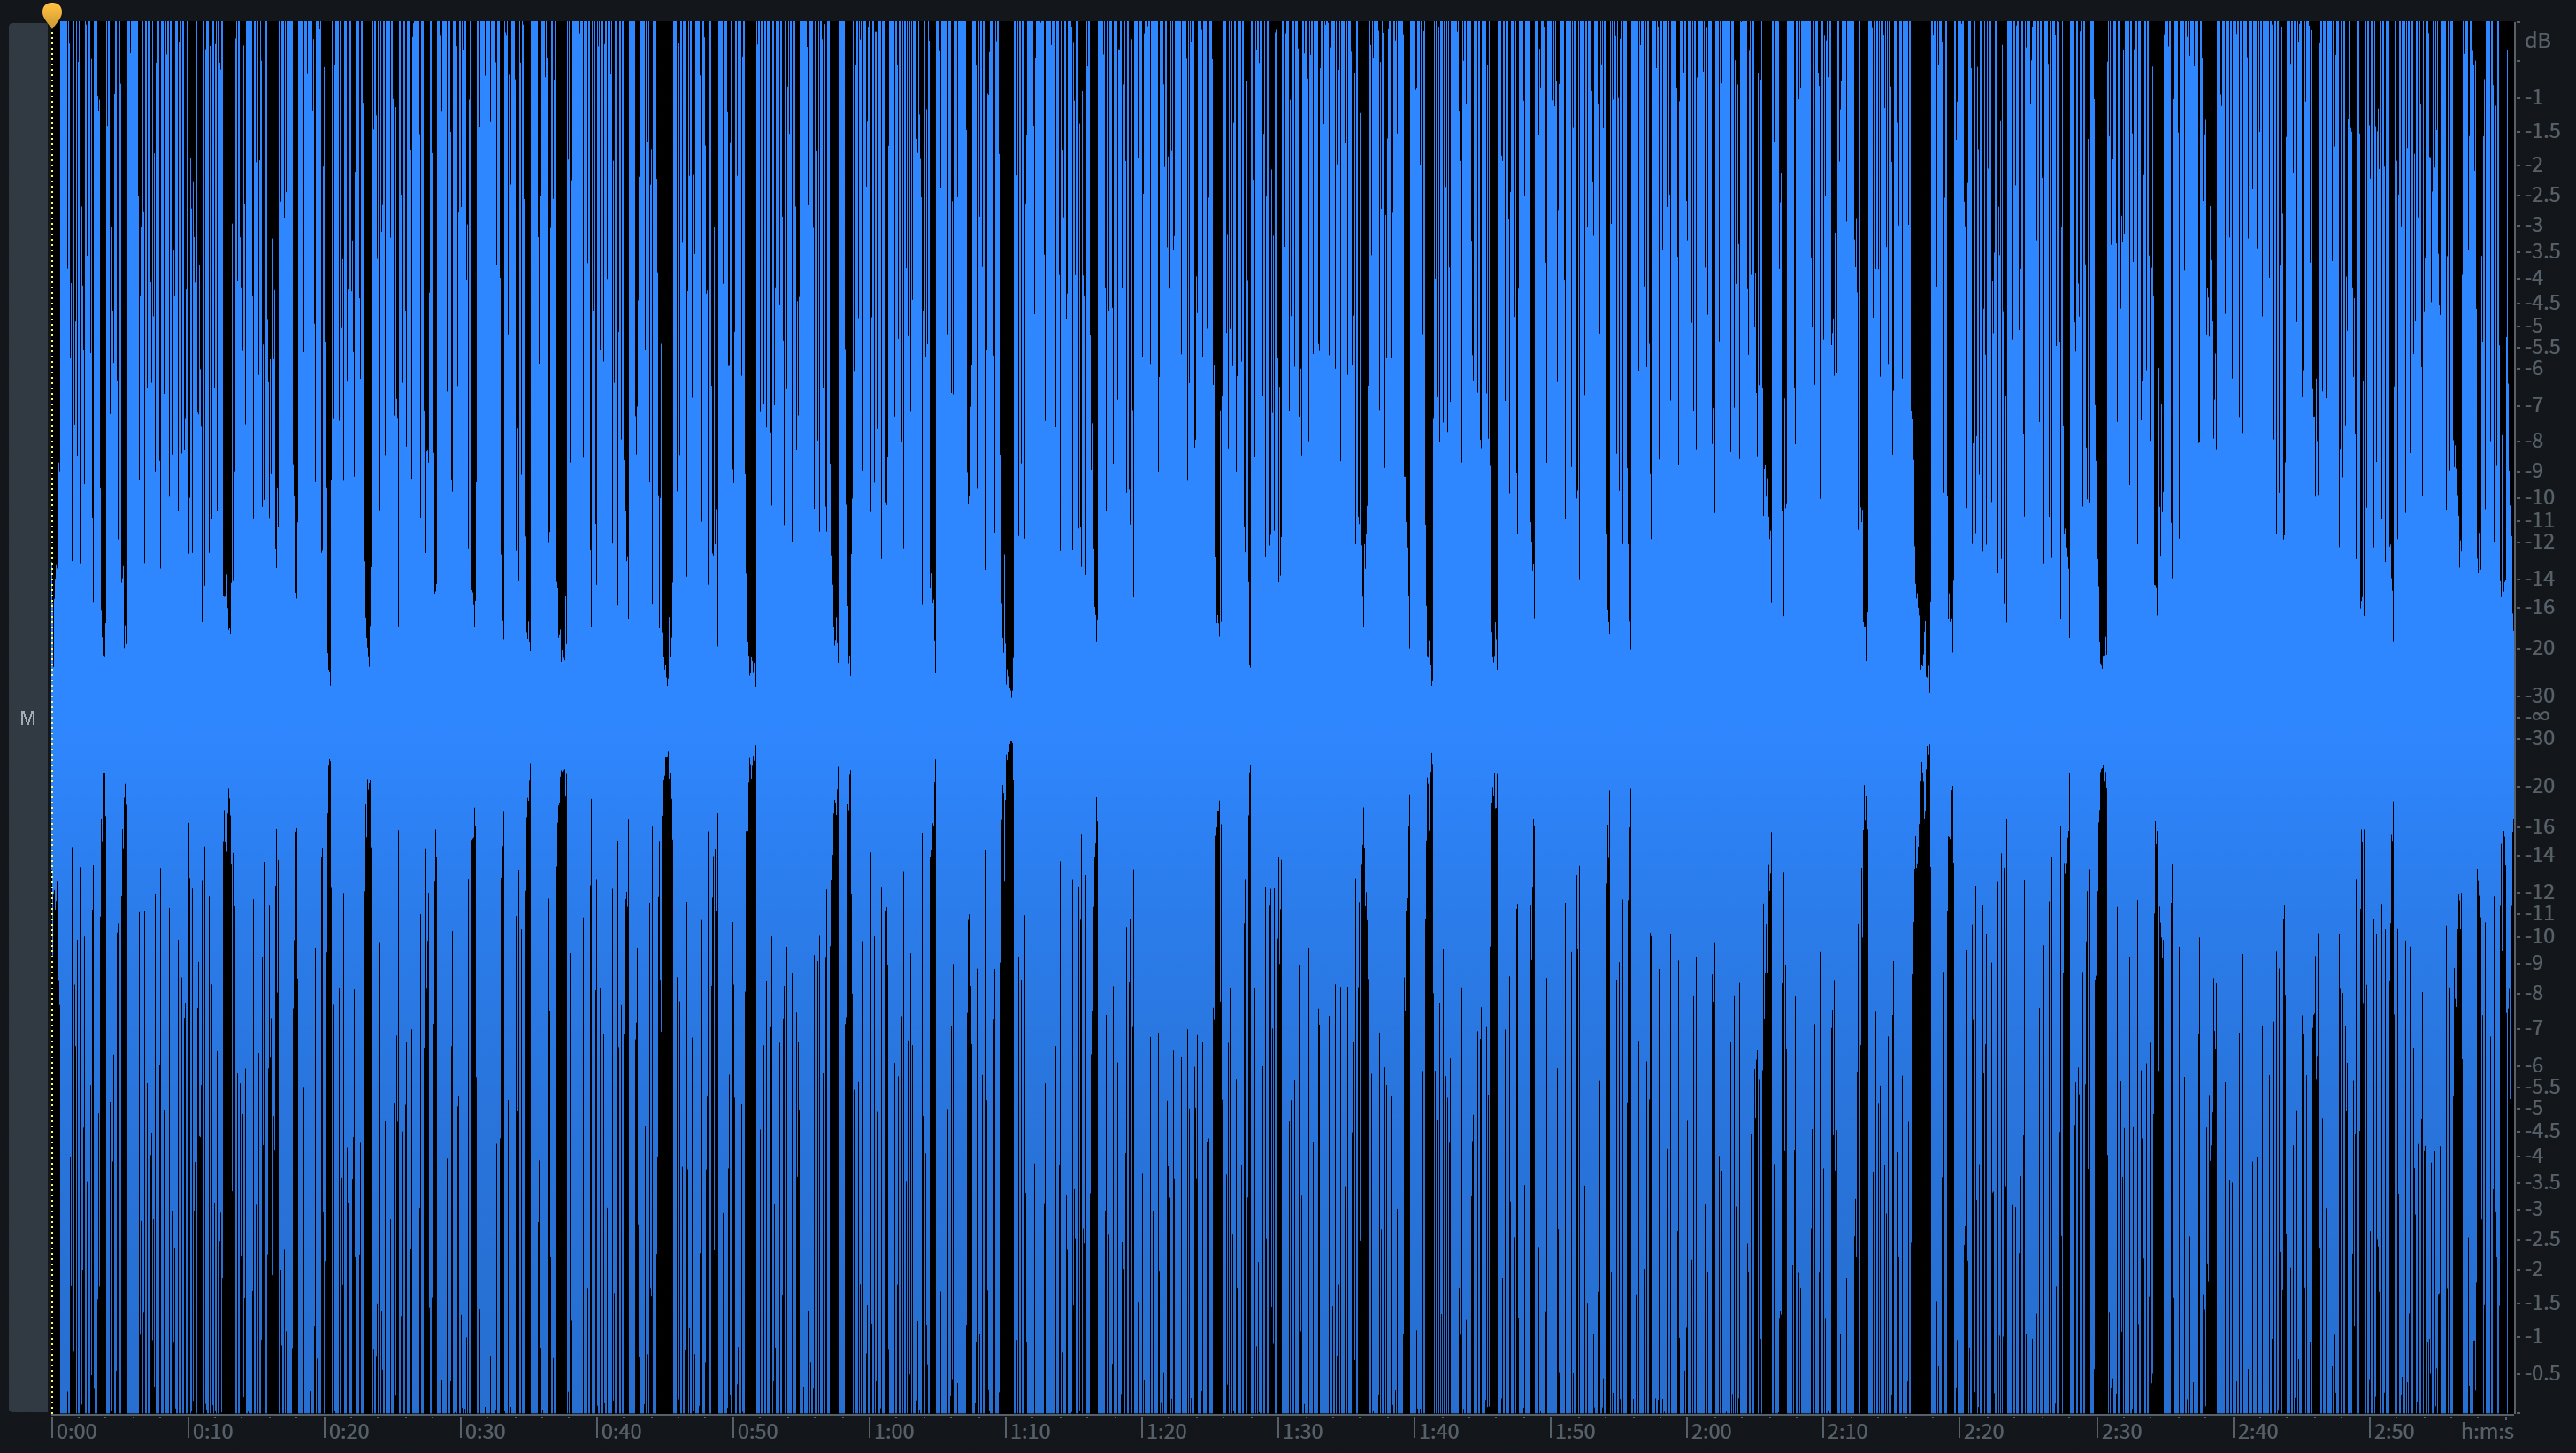
\includegraphics[width=\linewidth]{image/waveform_test1.png}
    \end{minipage}
    \begin{minipage}[t]{0.46\textwidth}
        \centering
        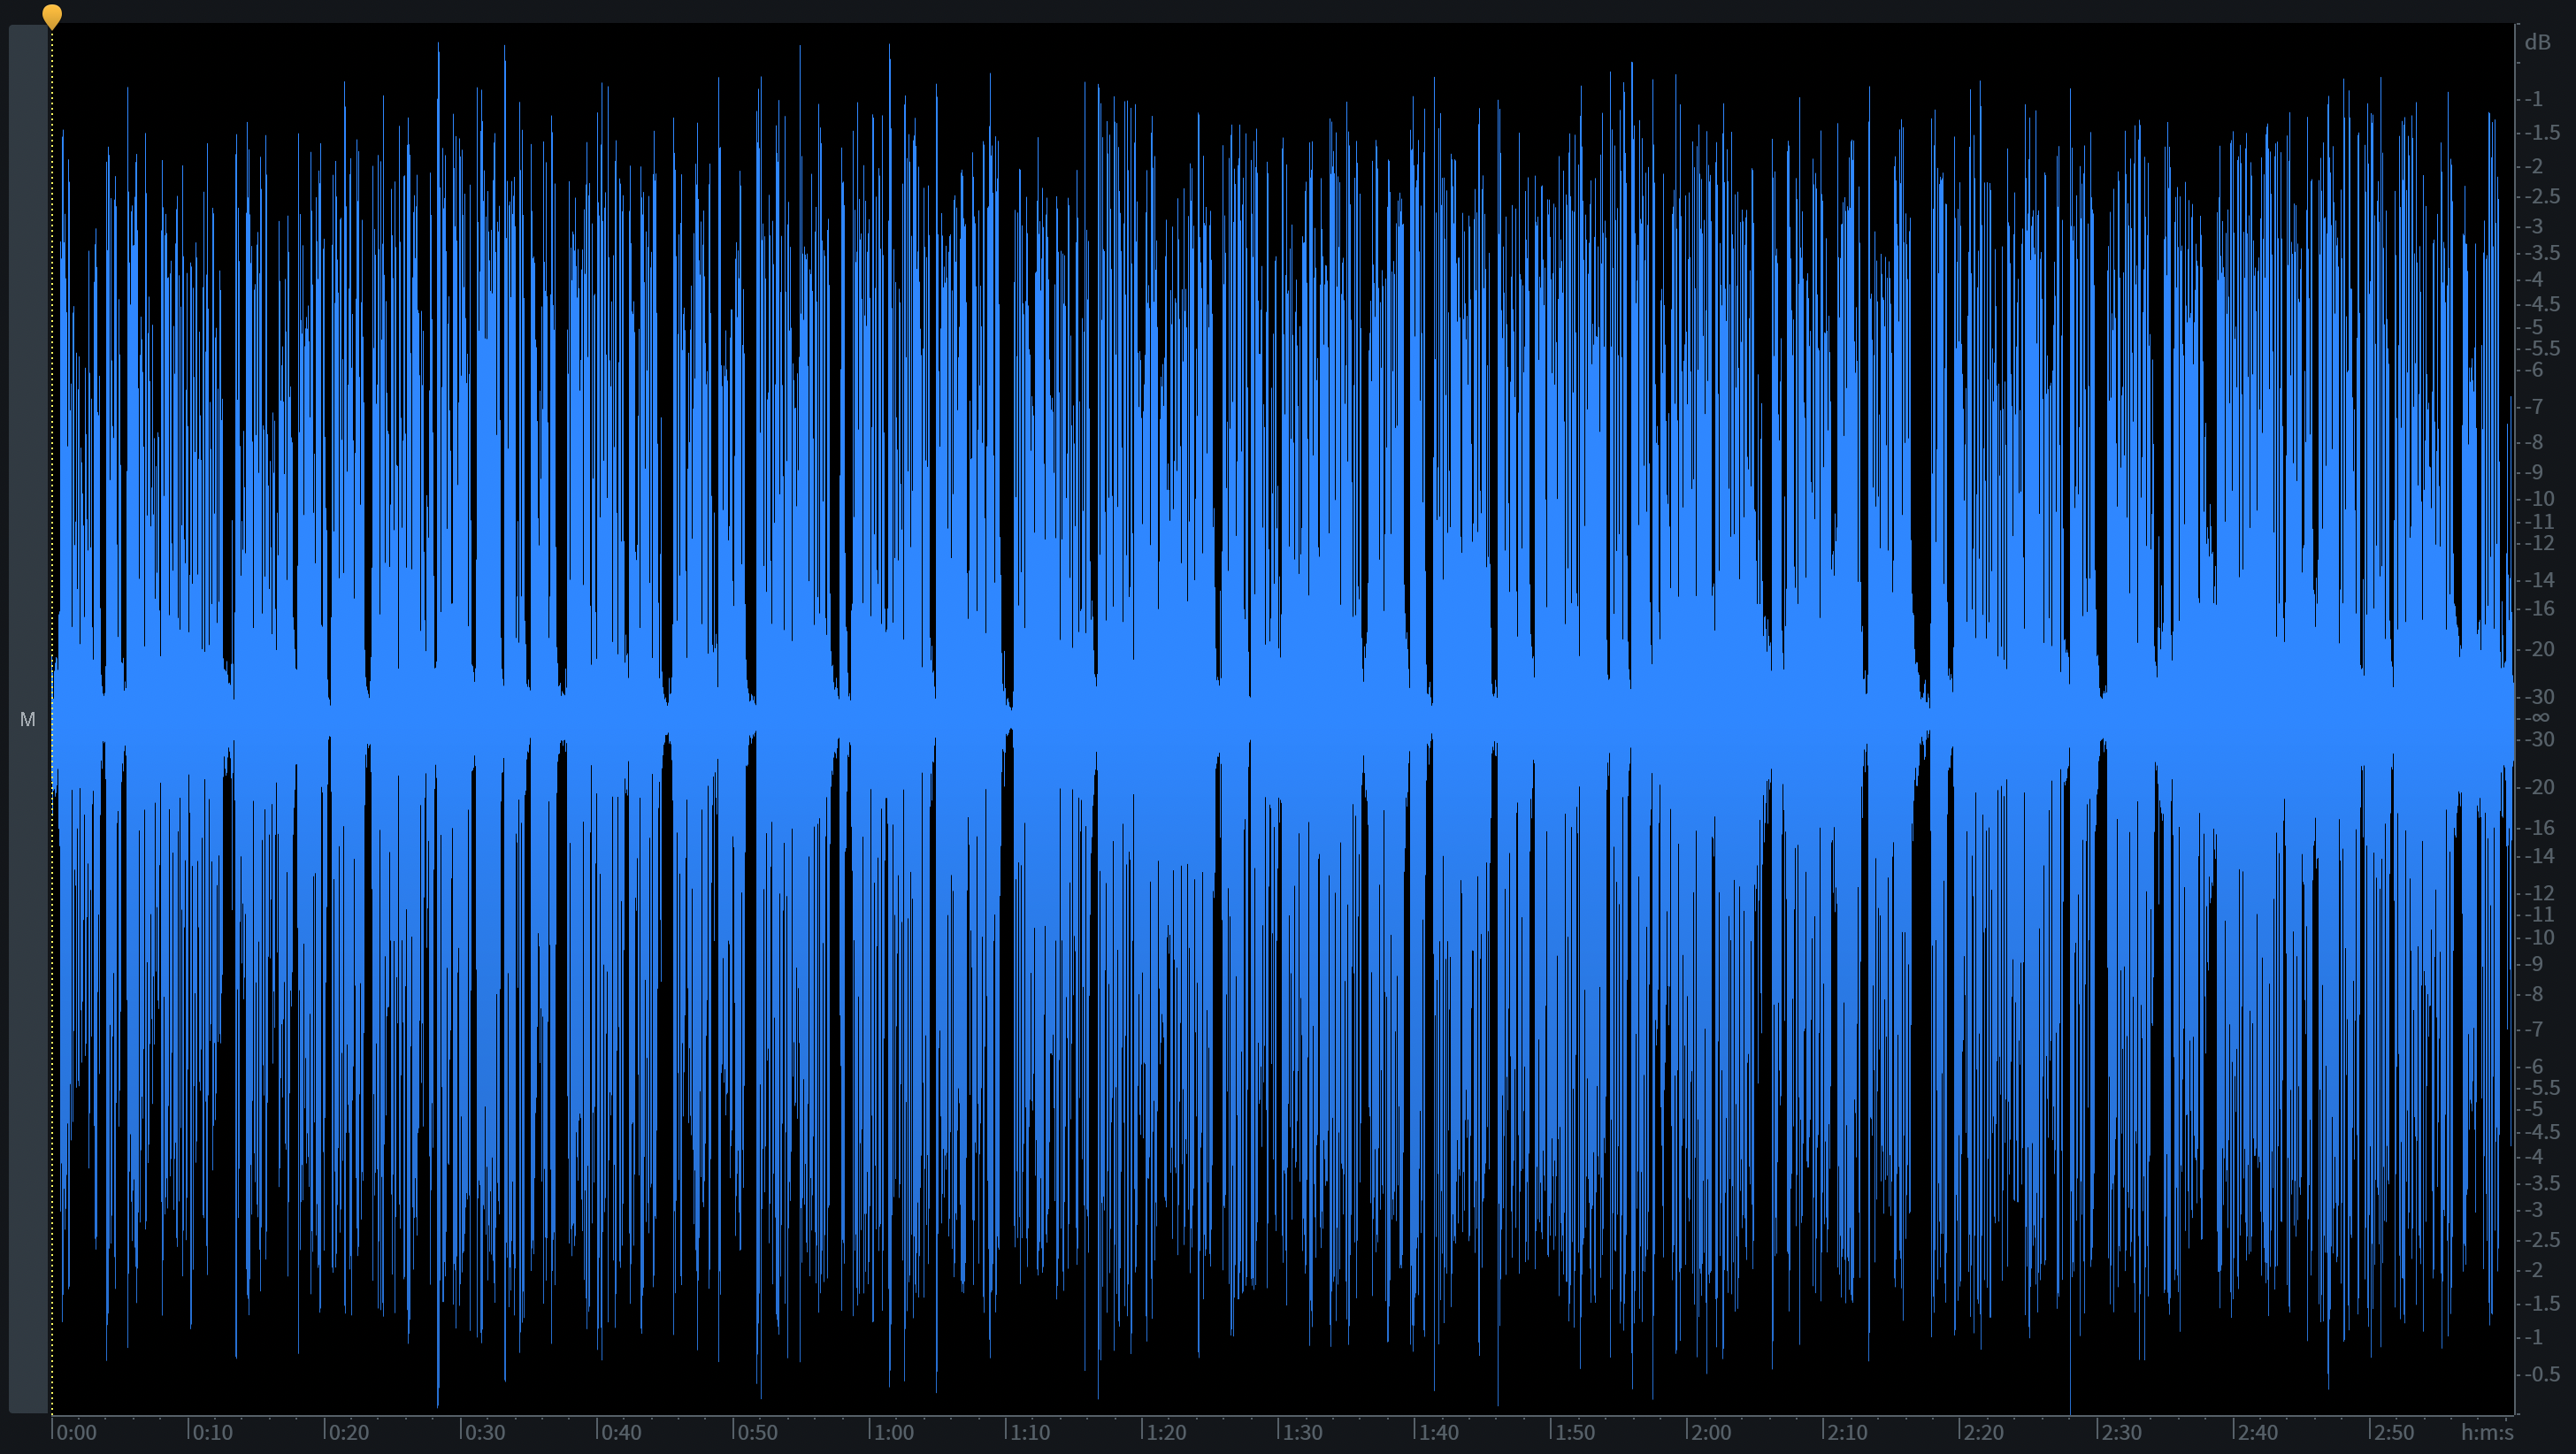
\includegraphics[width=\linewidth]{image/waveform_test2.png}
    \end{minipage}
    \captionWithStar{时域谱修复前后对比图}
\end{figure}

\subparagraph{时频谱比较} 时频谱(Spectrogram)又叫声谱图，它通过短时傅立叶变换，获取时间片段上的频率成分，以热图的形式将第三维的数值用颜色的深浅呈现出来。
如图\ref{时频谱修复前后对比图}所示，横坐标表示时间，纵坐标表示频率成分，颜色深浅表示该时间、频率区间下音频能量的大小。
对比修复前后的时频谱，我们可以明显看出，高频噪声明显减小，能量集中到人耳感知更强的频率范围。

\begin{figure}[htbp]
    \centering
    \begin{minipage}[t]{0.46\textwidth}
        \centering
        \includegraphics[width=\linewidth]{image/spectrogram_test1.png}
    \end{minipage}
    \begin{minipage}[t]{0.46\textwidth}
        \centering
        \includegraphics[width=\linewidth]{image/spectrogram_test2.png}
    \end{minipage}
    \captionWithStar{时频谱修复前后对比图}
\end{figure}


\paragraph{客观评价}
这里介绍两种常见的评价指标，分别是信噪比(Signal-Noise Ratio, SNR)、
与分段信噪比(Segmental SNR, SegSNR)。\cite{wavelet10}

\paragraph{信噪比(SNR):} 

\begin{equation}
    S N R=10 \lg \left[\frac{\sum_{n=1}^{L} s(n)^{2}}{\sum_{n=1}^{L}[s(n)-\hat{s}(n)]^{2}}\right]
\end{equation}

\paragraph{分段信噪比(SegSNR):}

\begin{equation}
    SegSNR=\frac{1}{M} \sum_{j=0}^{M-1} 10 \lg \left[\frac{\sum_{n=m j-N+1}^{m j} s^{2}(n)}{\sum_{n=m j-N+1}^{m j}\left[\hat{s}(n)-s(n)^{2}\right]}\right]
\end{equation}

由于语音信号是一种短时平稳信号，因此各个片段上的信噪比不同。
所以比起信噪比，分段信噪比更能反映语音去噪的性能。


\subsection{网络应用开发技术}

\hiddensubsubsection{AJAX}

AJAX是Asynchronous JavaScript and XML的简称，
指的是一套综合了多项技术的浏览器端网页开发技术，常被用于创建交互性能更强的应用程序。\cite{ajax3}
自2005年被Jesse James Garrett提出后，广泛的应用于Google包含Gmail，Gmap等产品中。

对比传统WEB应用中伴随表单提交的页面刷新，AJAX通过隐式更新数据的方法，让用户感知不到恼人的页面刷新。
且因为每次都是局部的数据更新，这使得服务器响应速度大大加快。

类似DHTML或者LNMP，AJAX并非一个固定的技术模块，\cite{ajax2}
而是一个开放式的技术框架，有机地利用了一系列相关技术，具有如下几条标准: 
\begin{enumerate}
\item 客户端(浏览器端)的界面展现使用HTML与CSS(层叠样式表)。
\item 数据采用XML/JSON格式存储与传输。
\item 客户端的数据请求通过HttpRequest对象封装。
\end{enumerate}


\hiddensubsubsection{jQuery}

jQuery是一套跨浏览器的高速、简洁的JavaScript库，可以用来简化HTML与JavaScript之间的操作，
是继Prototype之后的又一个优秀的JS框架。
jQuery倡导写更少量的代码，做更多的事情，或称为“Write less, Do more”。
具有下列特色: 
\begin{enumerate}
    \item 快速获取文档元素: jQuery实现了快速简明的查找DOM节点的功能，
    并提供了对链式操作的支持，大大提高了JS中获取页面元素的效率。
    \item 提供更强的异步处理能力: 使用Promise/Deferred模式更好的实现异步控制。
    \item 可以实现便利的网页补丁: 由于jQuery可以快速修改网页文本图像等内容，可以用来高效的实现网页的功能更新。
    \item 提供一系列工具: jQuery提供了JSON解析，特征检测，AJAX等工具函数。
\end{enumerate}

\hiddensubsubsection{Bootstrap}

Bootstrap是前端开发中最受欢迎的框架，用于开发响应式布局、移动设别有限的WEB项目。
包含阿里云官网、星巴克、Jupyter在内的众多大站都在其基础上开发。

它整合了常见的CSS布局组件和Javascript插件库，便于工程师们快速掌握和使用，极大的提高开发效率。
具有下列特色: 
\begin{enumerate}
\item 跨平台: 兼容Webkit、Chromium、Gecko等主流浏览器内核。
\item 提供全面组件: 提供全套美化过的UI组件供开发者使用。
\item 动态CSS: Bootstrap LESS让CSS彻底变成拥有很强逻辑性的标记语言。\cite{bootstrap1}
\end{enumerate}

\hiddensubsubsection{Django}

Django是一个Python驱动的高级Web应用框架，可以简化数据库驱动网站的开发。
由经验丰富的开发者创建并维护，为网站开发中最复杂的部分进行了模块化处理，帮助开发者快速便捷地创建高品质、易维护、数据库驱动的应用程序，
让专注于应用程序的编写，而不是疲弊于复杂的底层搭建。\cite{django2}
自2019年12月Django3.0发布以来，Django已经成为了最受开发者欢迎的MVC框架。

对比其它常见的Web框架，Django有如下优势: 
\begin{enumerate}
    \item 富内容: Django内建了完善的数据库封装和高效的后台管理机制，
    让开发者专注于内容创作。Django对比原始的网络开发，相当于Latex之于Word。
    \item 组件重用性: Django的设计理念是DRY(Don't Repeat Yourself)，
    最典型的例子是其强大、易扩展的Templates系统。\cite{django1}
    \item 热插拔: Django允许项目在运行中更改源码，可以实现更加灵敏的开发。
    \item MTV: Django使用MTV的方式实现了MVC理念，即模型(Model)、视图(View)和控制器(Controller)。
    由于Django自行处理了MVC中控制器的部分，因此开发者只需要关心模型(Model)、视图(View)和模版(Template)。
\end{enumerate}

\clearpage
\subsection{相关开发工具介绍}

\paragraph{Multipass}

Multipass 是一个轻量级虚拟机管理器，用于在任何平台上搭建高效Ubuntu虚拟机。
它在Linux上使用KVM、在Windows上使用Hyper-V、在MacOS上使用HyperKit，以便降低运行虚拟机的开销。
Multipass提供了便捷的命令行实现与虚拟机的交互，在Web开发这一不需要GUI的过程中，Multipass能够满足大部分开发者的需求。


\paragraph{Tampermonkey}

Tampermonkey是一种脚本管理器，用户可以通过脚本快速修改网页上的JavaScript。
其原理是在宿主页面加载完毕后，运行浏览器上的JS脚本，从而实现对浏览器渲染后的HTML的改变。
本项目使用这一工具辅助开发网站的测试功能。

\paragraph{Visual Studio Code}

Visual Studio Code 是一个开源轻量高颜值的跨平台编辑器，
不仅内置了JavaScript，TypeScript和Node.js的支持，还为其它语言与框架提供了丰富的扩展生态系统。
本项目的所有代码编写与论文排版都是在Visual Studio Code上完成。


\subsection{本章小结}
本章详细介绍了项目所需要的背景知识，包括如下三个部分: 
\begin{enumerate}
\item \emph{语音降噪的基础理论}: 介绍了语音信号的特点、噪声的类型、音频质量的评估标准。
\item \emph{网络应用开发部署技术}: 介绍了项目所使用的Web前后端技术，包括最流行的前端框架BootStrap，最适合快速交付的后端框架Django等。
\item \emph{相关开发工具介绍}: 介绍了虚拟机应用Multipass、前端测试工具Tampermonkey与代码编辑器Visual Studio Code。
\end{enumerate}


\clearpage
\section{音频修复理论与实现}

\subsection{音频信号多分辨率分析}

利用小波分析可以在语音信号的时频域上进行不同分辨率的研究，
比起傅氏分析，小波分析不仅能够处理平稳信号，还能很好的刻画非平稳信号，其产生具有划时代的意义。\cite{wavelet3}

\subsubsection{傅立叶分析}

\paragraph{傅立叶变换}
在小波分析还没出现之前，傅氏变换(Fourier Transform, FT)作为一种经典的语音信号处理方法，
一直受到广泛的关注和研究。它使用如下变换: 
\begin{align}
    \hat{f}(w) & =\frac{1}{\sqrt{2\pi}}\int_{-\infty}^{+\infty} f(t) e^{-j w t} d t
    \\
    f(t) & = \frac{1}{ \sqrt{2\pi}} \int_{-\infty}^{+\infty} \hat{f}(w) e^{j w t} d w
    \label{连续时间傅立叶变换}
\end{align}

实现了时域与频域之间的相互转换。

随着理论研究的深入，傅立叶分析的不足逐渐展现出来: 
在1873年，Reymond发现，$2\pi$周期函数的傅立叶级数不必点点收敛，而且即使收敛，它也未必收敛到原函数本身。

研究傅立叶变换的初衷是想将周期为$2\pi$的连续函数通过傅立叶分析转换为对应的傅立叶系数，
但现在发现原函数与其傅立叶系数没有严格的收敛和相等关系，那么这种研究方式就显得不合理。

最终，找到的适合傅立叶分析的函数类为Lebesgue建立的能量有限的$2\pi$周期函数类: 
\begin{equation}
    \mathcal{L}^2(0,2 \pi)=\left\{x(t) ; \int_{0}^{2 x}|x(t)|^{2} d t<+\infty\right\}
\end{equation}

对于分布参数与分布律不随着时间发生变化的平稳信号而言，
$\mathcal{FT}$提供了一种便捷的分析手段，
使得人们可以用相对简单的频谱特性来分析原本复杂的时间/空间信号的动态特性。

在工程上，为了计算及存储便利，我们采用其离散形式:
\begin{equation}
    \begin{array}{l}
    \tilde{x}[n]=\frac{1}{N} \sum_{k=0}^{N-1} \tilde{X}[k] e^{i \omega_{k} n}, \quad \omega_{k}=\frac{2 \pi k}{N} \\
    \tilde{X}[k]=\frac{1}{N} \sum_{n=0}^{N-1} \tilde{x}[n] e^{-i \omega_{k} n}
    \end{array}
\end{equation}
称为离散傅立叶变换(Discrete Fourier transform, DFT)。
在绘图时使用插值及归一化等技术手段，就能刻画出连续信号的采样序列的频谱性质。

在小波变换之前，傅立叶变换得到了广泛运用，
然而，因傅立叶变换的积分区间为$(-\infty,+\infty)$，所以它对频谱的描绘具有“全局性”，
无法反应时域局部特征，难以看出不同频率成分的信号产生与延续时间，这使得傅立叶分析无法运用到更加精密的分析中。

举例来说，当发生如图\ref{固定漂移$t=7$}所示的漂移时，我们需要分析工具解决两个问题: 

\begin{enumerate}
    \item 系统是否发生漂移?(漂移位置$t_0$)
    \item 发生了怎样的漂移?(漂移量$\delta$)
\end{enumerate}

\begin{figure}[htb]
    \centering
    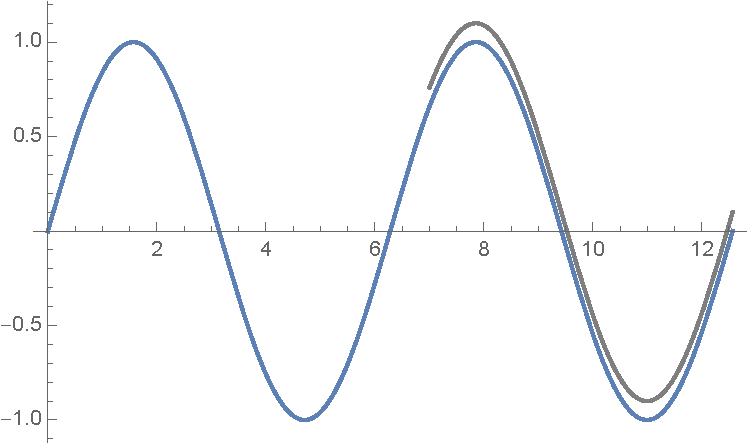
\includegraphics[width=0.7\textwidth]{image/section3/固定漂移.pdf}
    \captionWithStar{固定漂移$t=7$}
\end{figure}

我们直观的认为信号并没有发生太大的改变，只是被叠加了一个阶跃信号$g(t)$，发生了固定漂移$g(t) = \delta \cdot u(t-t_0)$。
然而只通过傅立叶分析却没有办法获得上述任意问题的解。


\paragraph{短时傅立叶变换}
由于傅立叶变换无法实现时间域的局部化分析，
这对包含音乐与语音在内的频域特性随着时间而变化的非平稳信号是非常不利的。\cite{wavelet6}

为了实现时域的局部化分析，Gabor提出了短时傅立叶变换(Short-Time Fourier Transform, STFT)，
基本思路是通过时间窗函数，将时间信号分成若干个小片段，对每一个片段独立进行傅立叶变换。

考虑到频谱计算时使用的($\mathcal{DFT}$)是由离散傅立叶级数($\mathcal{DFS}$)推导而成，
而$\mathcal{DFS}$要求原信号为周期序列，因此要求$\mathcal{DFT}$的序列首尾具有连续性。
对于短时傅立叶变换而言，使用均匀切分的时间片无法保证首尾的连续性，因此会造成泄漏现象。\cite{wavelet2}

举例来说，
对于只含有一个频率元素的三角函数信号而言，如果片段的长度不是周期的整数倍，频谱图上就会出现不止一个尖峰。

于是，我们需要通过平滑片段的开始和结尾来缓解其不连续性，从而减少泄漏，这种方法就是加窗。
最终，短时傅立叶变换的表达式为: 
\begin{equation}
    S(w, \tau)=\int_{-\infty}^{+\infty} f(t) g^{*}(t-\tau) e^{-j w t} d t
\end{equation}
其中，$g(t)$代表窗函数，常见的有矩形窗，汉明窗等。

将$\mathcal{STFT}$可视化的方法有很多种，最为通用的是图\ref{时频谱}所示的时频谱。

为了使得时频谱尽可能清晰，需要同时提高时频分辨率。
然而时间分辨率随着片段的增长而降低；频率分辨率却随着片段的增长而升高。
这一限制被称为\emph{Gabor限制}，它是这类时频分析的基础限制。\cite{wavelet1}

Gabor限制揭示了短时傅立叶变换的固有缺点，即它存在分析上的矛盾:

一方面，$\mathcal{STFT}$在选择完窗函数并确定片段长度后，时频谱就已经确定，
与每个区间的频率成分毫无关系。

另一方面，我们直观的认为，由于高低频对时域的作用力不同，对于高频成分，时间间隔要选取的尽量小，这样采样率会增高，从而提高获取的波形精度，进而更好的确定峰值，就需要更窄的“窗”；
对于低频成分，由于波形较宽，时间段需要足够长才能给出完整的数个周期，才能给出完整信息，所以时间间隔需要扩大，即需要更宽的“窗”。

综上需要选取一个灵活的时频“窗口”，能够在高频区间自动缩小窗口宽度，在低频区间自动扩大窗口宽度，
这一需求被称为多分辨率分析。

\begin{figure}[htbp]
    \centering
    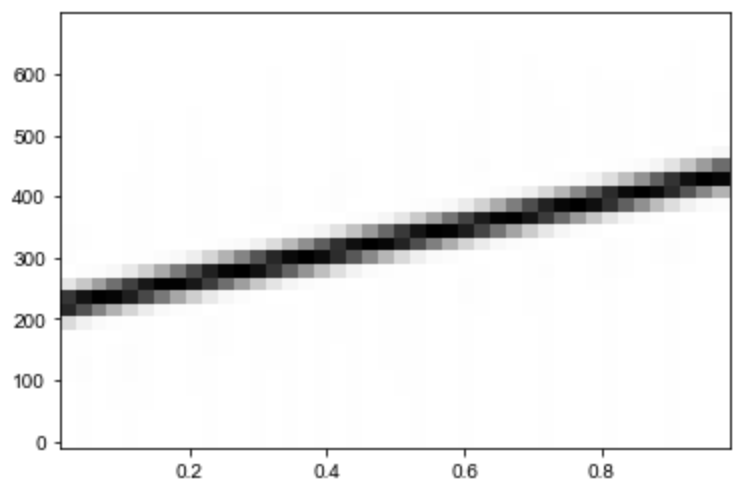
\includegraphics[width=\textwidth]{image/section3/时频谱.png}
    \captionWithStar{时频谱}
\end{figure}

\paragraph{傅氏分析局限性的原因分析}

\begin{enumerate}
    \item \emph{从基的角度}: 待分析的信号属于信号空间$\mathcal{L}^2(\mathbb{R})$，
    但是分析工具选用的基$e^{iwt}$却不属于平方可积这一信号空间，
    因而无法很好的体现待分析对象与分析工具间的相关性。
    \item \emph{从计算角度}: 依据$\mathcal{IFT}$的表达式可以看出，一旦$w$产生了偏差，重构的原信号$f(t)$就截然不同
    也就是说不同的频率成分需要用$\mathcal{FT}$严格的区分开。
    但在现实计算中，无法保证$\mathcal{FT}$的无偏，且因为选用了$e^{iwt}$作为基，即便$\hat{f}(\omega)$控制得很好，
    重构回的信号也会差得很远。\cite{wavelet4}
\end{enumerate}

\clearpage
\subsubsection{小波分析}

\paragraph{连续小波}

由上文可知，傅立叶分析在时域局部化上存在局限性的根本原因就是基的选择不恰当。
因此，小波要想解决这一问题，就需要选用更加恰当的基，如果$\psi(t)$满足下面两个条件: 
\begin{enumerate}
\item $\psi(t) \in \mathcal{L}^{2}(\mathbb{R})$
\item $C_{\psi}=\int_{-\infty}^{+\infty} \frac{|\hat{\psi}(\omega)|^{2}}{\mid \omega \|} d w<+\infty$
\end{enumerate}
则称$\psi(t)$为小波基(母函数)。

对小波母函数进行相应变换就可以获得依赖参数a,b的连续小波，简称小波:
\begin{equation}
    \psi_{a, b}(t)=\frac{1}{\sqrt{a}}\left(\frac{t-b}{a}\right)
    \label{依赖参数a,b的连续小波}
\end{equation}
其中$a\ne 0, b \in \mathbb{R}$，分别代表尺度因子和平移因子。

如果语音信号$f(t) \in \mathcal{L}^{2}(\mathbb{R})$，就可以对$f(t)$使用连续小波变换(CWT):\cite{wavelet7}
\begin{equation}
    W_{f}(a, b)=<f(t), \psi_{a, b}(t)>=\frac{1}{\sqrt{a}} \int_{-\infty}^{+\infty} f(t) \psi^{*}\left(\frac{t-b}{a}\right) d t
\end{equation}

其反变换为
\begin{equation}
    f(t) = \frac{1}{C_\psi} \iint_{R\times R^{*}}W_{f}(a,b)\psi_{a,b}(t)\frac{d a d b }{a^{2}}
\end{equation}

这个公式很好的体现了不同尺度因子的小波系数对原信号的重要性差异: 
固定b的情况下，$a$越接近0，对应的小波系数$W_{f}(a,b)$对应的权值($\frac{d a d b }{a^{2}}$)越高，
即在重建的过程中，贡献越大。

通过这个公式，还可以得出一个$\mathcal{WT}$与$\mathcal{FT}$在数值计算上的不同: 
傅立叶变换中，每个成分同等重要，都要保证极高的精确度，需要等间隔的取积分值；
而小波变换中，尺度因子越接近0，越要保持较高的精确度，不能等间隔的取积分值。

由于小波变换是一个升维分析，大大提高了计算量，在实际运用中非常不方便。
为了减少工作量，可以考虑对待分析的信号或者分析工具使用的基做限制。
出于分析域的完整性考量，不同于傅立叶分析，小波分析中选择限制基。

\paragraph{吸收小波} 
首先对尺度因子的非负性做出限制，如果$\psi(t)$满足
$
\int_0^{+\infty}\frac{|\hat{\psi}(\omega)|^{2}}{\omega}d \omega = \int_0^{+\infty}\frac{|\hat{\psi}(-\omega)|^{2}}{\omega}d \omega
$，
则称$\psi(t)$为吸收小波，那么反变化可表达为: 
\begin{equation}
    f(t) = \frac{2}{C_\psi} \int_0^{+\infty} \int_{-\infty}^{+\infty}W_{f}(a,b)\psi_{a,b}(t)\frac{d a d b }{a^{2}}
\end{equation}

为了进一步较小尺度因子的分析量，希望$a$能取离散值；
由于前面的分析，$a$显然不能均匀取值，所以希望通过$a$的对数取值实现离散化。

\paragraph{二进小波}
$\psi(t)$ 满足
$
0<A \leqslant \sum_{j=-\infty}^{+\infty}\left|\hat{\psi}\left(2^{-j} w\right)\right|^{2} \leqslant B<+\infty, a.e, w\in \mathbb{R}
$(几乎处处成立)，
则称$\psi(t)$是二进小波，那么逆变换公式写作:  
\begin{equation}
    f(t)=\sum_{j =-\infty}^{+\infty} 2^{j} \int_{-\infty}^{+\infty}  W_{f}\left(2^{-j}, b\right)\tau_{2^{-j},b}(t)d b
\end{equation}
其中$\tau(t)$满足
$
\sum_{i=-\infty}^{+\infty} \bar{\hat{\psi}}\left(2^{-j} w\right) \hat{\tau}\left(2^{-j} w\right) \equiv 1 , a.e, w \in \mathbb{R}
$，称为“重构小波”。

显然，根据$\psi(t)$与$\tau(t)$的谱关系，很容易找出$\tau(t)$，即
\begin{equation}
\hat{\tau}(w) = \hat{\psi}(w)/\sum_{j\in R}|\hat{\psi}(2^{-j}w)|^2
\end{equation}

至此，尺度因子$a$已经用2的整数次幂离散化了，但平移因子$b$仍然是连续取值的，
为了让$b$也能离散化，还需要对基加以更严厉的限制；
此外，二进小波正变化与逆变换使用的基是不同的，希望能够通过进一步限制基，使这二者相同。


\paragraph{正交小波}
若 
$
\left\{\psi_{j, k}(t)=2^{j/2} \psi(2^{j}t-k), (j,k) \in \mathbb{Z}^2\right\}
$
构成$\mathcal{L}^2(\mathbb{R})$的标准正交基(O.N.B)，
则称$\psi(t)$是正交小波，
根据线性代数的知识，可知: 
\begin{equation}
f(t)=\sum_{j=-\infty}^{+\infty} \sum_{k=-\infty}^{+1 \infty} \alpha_{j, k} \psi_{j, k}(t)
\end{equation}

其中， $\alpha_{j,k} = \Braket{f(t),\psi_{j,k}(t)} = W_{f}(2^{-j},2^{-j}k)$  

由此可得: 
\begin{equation}
    f(t)=\sum_{j=-\infty}^{+\infty} \sum_{k=-\infty}^{+1 \infty} W_{f}(2^{-j},2^{-j}k) \psi_{j, k}(t)
\end{equation}


因此: 只要$\psi(t)$是一个正交小波，
那么分析$f(t)$的时域性质就可以转化为分析$f(t)$在正交小波变换上对应尺度参数$j$与平移参数$k$的小波系数。


\paragraph{离散序列的小波分解与重构}
$\mathcal{DWT}$对不同频段不同分辨率的信号进行分析，将信号分解为粗略近似和细节信息，如图\ref{滤波分析图}所示：

\begin{figure}[htbp]
    \centering
    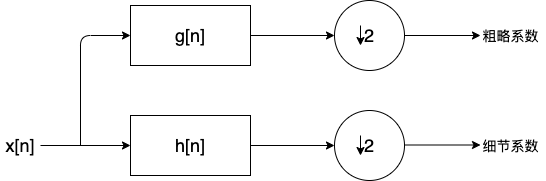
\includegraphics[width=0.8\textwidth]{image/section3/滤波分析图.png}
    \captionWithStar{滤波分析图}
\end{figure}
信号$x[n]$的DWT是通过一系列滤波器计算出来的。

首先将连续信号的离散采样点$x[n]$通过单位脉冲响应为$g[n]$的低通滤波器，
生成的信号为这二者的卷积，如式\ref{经过低通滤波器}所示: \cite{wavelet5}

\begin{equation}W
    y[n]=(x * g)[n]=\sum_{k=-\infty}^{\infty} x[k] g[n-k]
    \label{经过低通滤波器}
\end{equation}

同时，使用高通滤波器对信号进行分解。
如此可以生成高通滤波器的细节系数和低通滤波器的近似系数。
需要提及的是，这两个滤波器必须是相关的(称为“正交镜像滤波器”)，如式\ref{正交镜像滤波器}。
由于现在已经去掉了一半频率，根据Nyquist法则，可以丢掉一般的样本。

\begin{equation}
    \begin{array}{l}
    y_{\text {high }}[n]=\sum_{k=-\infty}^{\infty} x[k] h[2 n-k] \\
    y_{\text {low }}[n]=\sum_{k=-\infty}^{\infty} x[k] g[2 n-k]
    \end{array}
    \label{正交镜像滤波器}
\end{equation}

这种分解方式使时间分辨率降低了一半，因为每个滤波器输出只有一半的信号特征。 
然而，每个输出有输入的一半频段，所以频率分辨率提高了一倍。

重复进行这种分解，进一步提高频率分辨率， 
并用高低通滤波器对近似系数进行分解，然后进行下采样。
这以二进制树的形式表示，节点代表不同时频定位的子空间。
这种树被称为滤波库。

\begin{figure}[htbp]
    \centering
    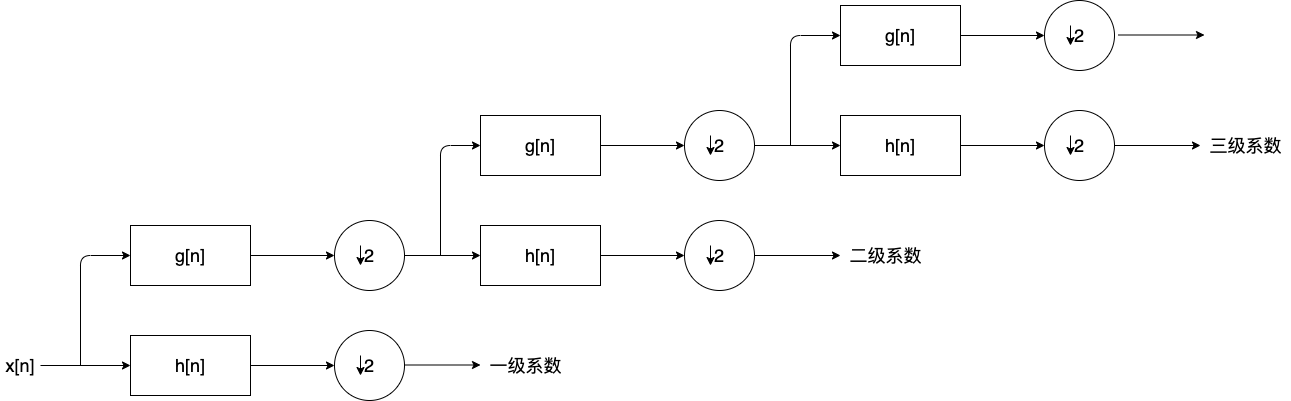
\includegraphics[width=\textwidth]{image/section3/三级滤波库.png}
    \captionWithStar{三级滤波库}
\end{figure}

如图\ref{三级滤波库}，每一层级的信号都被分成高频和低频成分。
由于是分解过程，所以信号的采样点必须是$2^N$，其中$N$是分解的级数。


\subsection{小波阈值去噪算法实现}

考虑到有用信号的小波系数通常集中在低频，而噪声信号的小波系统一般集中在高频。
所以选用某个\emph{小波基}对音频信号信号进行多尺度分析时，随着分解层数的提高，噪声的小波系数越来越小。
小波阈值降噪就是利用这一特性，到一定\emph{分解层数}时，设定一个\emph{阈值}，
认为阈值以下的小波系数对应的是高频噪声，需要使用一定的\emph{阈值函数}滤除或压缩；
而阈值之上的就是有用信号，需要保留或增强。
之后用处理完成后的小波系数重建音频，从而达到语音增强的目的。\cite{wavelet8}


\subsubsection{分解层数设置}
因为待处理的是语音信号，频率区间为300-3000Hz，而现在主流的音频文件都是$44100$Hz的采样率(约为$44000$)
由于mallet每次都是抽二分层，采样率下降一半，所以频率如图\ref{分解层数}所示:  

\begin{figure}[htbp]
    \centering
    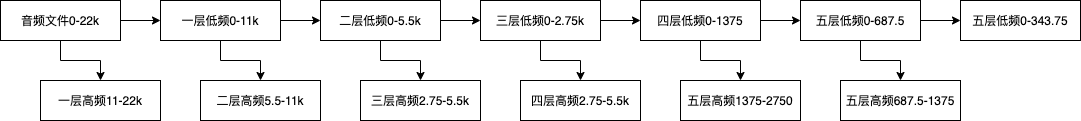
\includegraphics[width=\textwidth]{image/section3/分解层数.png}
    \captionWithStar{分解层数}
\end{figure}

可以看到第五层的低频已经分解到了$343.75Hz$了，再次分解显然没有必要了，因此分解层数确定为五层。

\subsubsection{阈值确定}
阈值的选择直接影响了小波阈值降噪的性能。
如果选择的阈值太小，噪声成分就会被保留；如果选择的阈值过大，有用信号就会被破坏，造成信号的失真。
目前有三种常见的阈值选择方法: 通用阈值、无偏似然阈值、启发式阈值还有极值阈值估计: 

本文选用通用阈值，表达式如式\ref{通用阈值}: 

\begin{equation}
    Th_{j}=\sigma \sqrt{2 \ln (N)} / \ln (j+1)
    \label{通用阈值}
\end{equation}

其中，$N$表示信号长度，$\sigma$表示噪声标准差，$j$表示当前所在层数。

\begin{enumerate}
\item 由于本项目只是一个针对音频的在线修复系统，无法确定噪声的性质，因此采用估计值$\operatorname{median}\left(\left|w_{j, k}\right|\right) / 0.6745$。
\item 由于多尺度分析中每一层的噪声与有用信号的比例不同，采用一个与所在分解层数无关的阈值是不合理的，所以在式\ref{通用阈值}的分母上添加$\ln (j+1)$。
当所在层数增大时，阈值会响应减小，更有利于低频有用信号的保留。
\item 对比其它几种阈值，通用阈值计算简单，物理意义明确。
\end{enumerate}


\subsubsection{小波基选择}
小波基函数的选取主要由四个因素确定，分别是：支撑长度、消失矩、正则性以及相似性。

\begin{enumerate}
\item \emph{支撑长度}: 如果FIR小波滤波器的长度为$N$，那么支撑长度就是$N-1$。
也就是说支撑长度越长，计算量越大。

\item \emph{消失矩}: 用来表示小波母函数向无穷衰减的方式，
如果$\psi(t)$的消失矩为$p$，那么： 
\begin{equation}
    \int_{-\infty}^{+\infty} t^{k} \psi(t) d t=0 \text { for } 0 \leq k<p
\end{equation}
也就是说$\psi(t)$与$p$阶以下的原始信号都正交。
如果消失矩$p$越大，说明与之正交的阶数越多，就表示大的小波系数更集中在一个小频率段中，
也就意味着高频子带带小波系数越小。
此外，消失矩越大，小波母函数的震荡越多。

\begin{figure}[htbp]
    \centering
    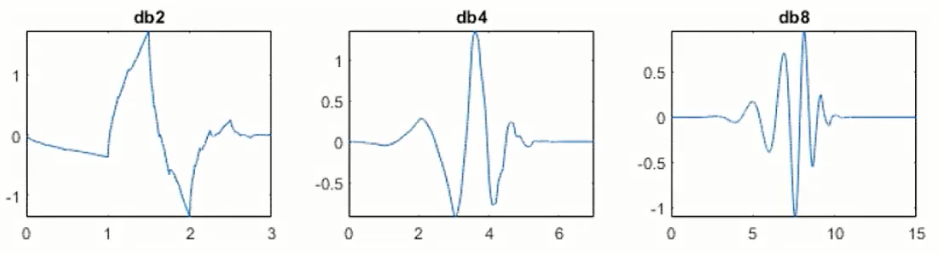
\includegraphics[width=\textwidth]{image/section3/消失矩.png}
    \captionWithStar{消失矩}
\end{figure}

\item \emph{正则性}: 描述小波基存在的连续导数的阶数，正则性越好，重构的小波越光滑，越能减小人耳对重构误差的感知。

\item \emph{正交性}: 根据线性代数的知识，正交性越好，重构的误差越小，分解小波变换越能保全能量，有利于小波逆变换。

\end{enumerate}



本项目的主要需求是降噪，因此在信号重建中保留能量是最重要的，所以最后选择在正交性上最严密Daubechies小波族。\cite{wavelet1}
此外，我们还同时希望选择的小波基紧支撑(支撑长度短)和光滑(正则性好)，由于这两点是矛盾的，在权衡利弊后选择了Daubechies7小波基。

\subsubsection{阈值函数设计}
根据上文中所说，需要将低于阈值$Th$的小波系数看作噪声，使用阈值函数去除。
这一步是否高效，很大程度上依赖于就是看阈值函数的设计。
在目前的文献中，适用于语音处理的阈值技术主要有两种，即硬阈值和软阈值。


\paragraph{硬阈值}

硬阈值可以描述为将绝对值低于阈值的元素直接置零。
令$T_h$为给定阈值，那么硬阈值去噪可定义为:
\begin{equation}
    {w'}_{j, k}=\left\{\begin{array}{ll}
    w_{j, k} & \left|w_{j, k}\right| \geq Th \\
    0 & \left|w_{j, k}\right|<Th
    \end{array}\right.
\end{equation}

硬阈值的缺陷在于不连续，重建后的波形会出现严重的吉布斯效应。

\paragraph{软阈值}

软阈值是硬阈值不连续问题的一种解决方式，具体方法是先将绝对值低于阈值的元素设为零，再让非零系数向零收缩。

软阈值去噪可定义为:

\begin{equation}
    {w'}_{j, k}=\left\{\begin{array}{cl}
    \operatorname{Sign}\left(w_{j, k}\right)\left(\left|w_{j, k}\right|-Th\right) & \left|w_{j, k}\right| \geq Th \\
    0 & \left|w_{j, k}\right|<Th
    \end{array}\right.
\end{equation}

可以明显看出，软阈值函数虽然避免了阈值附近的不连续，但对处理后的小波系数的绝对值莫名的被减小了一个$Th$，
意味着原始信号中的有用信息很可能收到了损失。


\paragraph{软硬折中阈值}

对软阈值进一步修改，调整$Th>0$的情况，可以得到新的阈值函数: 

\begin{equation}
    {w'}_{j, k}=\left\{\begin{array}{cc}
    \operatorname{sign}\left(w_{j, k}\right)\left(\left|w_{j, k}\right|-\alpha Th\right) & \left|w_{j, k}\right| \geq Th \\
    0 & \left|w_{j, k}\right|<Th
    \end{array}\right.
    \label{软硬折中阈值}
\end{equation}

其中，$\alpha$为可调参数($\alpha \in [0,1]$)。

如图\ref{三种阈值方法的比较}所示: 
这个阈值法虽然减轻了影响但没能根本的解决问题，后续的研究中仍然
需要寻找一个既连续又能较好的保持阈值以上小波系数不变(即渐近线为$y=x$)的阈值函数。

\begin{figure}[htb]
    \centering
    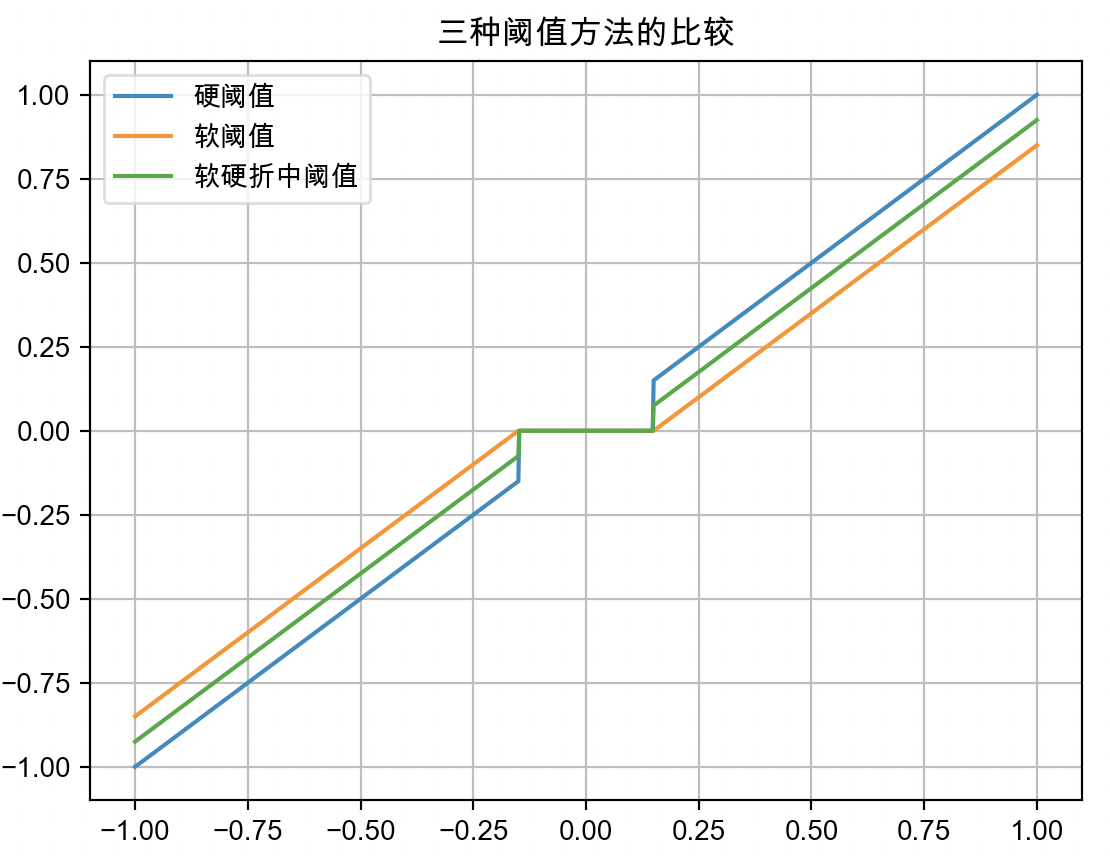
\includegraphics[width=0.65\textwidth]{image/section3/三种阈值方法的比较.png}
    \captionWithStar{三种阈值方法的比较}
\end{figure}


\subsection{仿真分析}

本次实验使用Python完成，原始语音文件通过you-get从获取网络获取视频，
再通过moviepy实现音频的提取。本实验控制为两个变量:信噪比与阈值函数。
信噪比从-5到15dB，阈值函数分别使用上文介绍的软、硬和软硬折中函数。其余变量保持不变：
\begin{enumerate}
\item \emph{小波基}: 因为在仿真阶段，不太重视计算量，所以选择支撑长度较大的小波基，最后选用Db7小波基；
\item \emph{分解层数}: 由于moviepy提取出来的音频采样率设置为44100Hz，所以根据上文的分析，最终采用五层分解；
\item \emph{阈值}: 考虑形式和物理意义的直观，使用通用阈值；
\end{enumerate}

\begin{table}[htb]
    \centering
    \captionWithStar{测试音频一}
    \begin{tabular}{|p{3cm}|p{3cm}|p{3cm}|p{3cm}|}
    \thickhline
    \textbf{信噪比(dB)} & \textbf{软阈值} & \textbf{硬阈值} & \textbf{软硬折中阈值} \\
    \thickhline
    -5               & 2.4371       & 2.0838       & 2.5575          \\
    \hline
    0                & 5.7453       & 6.0215       & 6.2971          \\
    \hline
    5                & 8.4205       & 9.7833       & 9.6444          \\
    \hline
    10               & 10.5024      & 12.8925      & 12.3175         \\
    \hline
    15               & 12.1679      & 15.5763      & 14.4933         \\
    \thickhline
    \end{tabular}
\end{table}

\begin{table}[htb]
    \centering
    \captionWithStar{测试音频二}
    \begin{tabular}{|p{3cm}|p{3cm}|p{3cm}|p{3cm}|}
    \thickhline
    \textbf{信噪比(dB)} & \textbf{软阈值} & \textbf{硬阈值} & \textbf{软硬折中阈值} \\
    \thickhline
    -5               & 0.9138       & 0.4826      & 1.4783          \\
    \hline
    0                & 2.8881       & 2.9258       & 4.2612          \\
    \hline
    5                & 5.8540       & 6.1543       & 7.5257          \\
    \hline
    10               & 9.6715      & 10.3729      & 11.5531         \\
    \hline
    15               & 13.4355      & 14.5732      & 14.9753         \\
    \thickhline
    \end{tabular}
\end{table}

\begin{table}[htb]
    \centering
    \captionWithStar{测试音频三}
    \begin{tabular}{|p{3cm}|p{3cm}|p{3cm}|p{3cm}|}
    \thickhline
    \textbf{信噪比(dB)} & \textbf{软阈值} & \textbf{硬阈值} & \textbf{软硬折中阈值} \\
    \thickhline
    -5               & 0.7949       & 1.2499       & 1.4356          \\
    \hline
    0                & 4.0203       & 5.4250       & 5.2838          \\
    \hline
    5                & 7.2648       & 9.0119       & 8.6717          \\
    \hline
    10               & 9.8402      & 11.5976      & 11.1931         \\
    \hline
    15               & 11.7402      & 13.4875      & 13.0693         \\
    \thickhline
    \end{tabular}
\end{table}

\begin{table}[htb]
    \centering
    \captionWithStar{测试音频四}
    \begin{tabular}{|p{3cm}|p{3cm}|p{3cm}|p{3cm}|}
    \thickhline
    \textbf{信噪比(dB)} & \textbf{软阈值} & \textbf{硬阈值} & \textbf{软硬折中阈值} \\
    \thickhline
    -5               & 1.6754       & 1.2832       & 2.0179          \\
    \hline
    0                & 4.3167       & 4.4736       & 5.2791          \\
    \hline
    5                & 7.1372       & 7.9688       & 8.5850          \\
    \hline
    10               & 10.0869      & 11.6327      & 11.9353         \\
    \hline
    15               & 12.8017      & 15.0747      & 14.7343         \\
    \thickhline
    \end{tabular}
\end{table}

\begin{table}[htb]
    \centering
    \captionWithStar{测试音频五}
    \begin{tabular}{|p{3cm}|p{3cm}|p{3cm}|p{3cm}|}
    \thickhline
    \textbf{信噪比(dB)} & \textbf{软阈值} & \textbf{硬阈值} & \textbf{软硬折中阈值} \\
    \thickhline
    -5               & 1.7087       & 1.7325       & 2.9139          \\
    \hline
    0                & 6.9084       & 8.3508       & 9.545           \\
    \hline
    5                & 13.1188      & 15.1662      & 16.1974         \\
    \hline
    10               & 19.5117      & 21.9705      & 22.7462         \\
    \hline
    15               & 25.1757      & 28.0607      & 28.0446         \\
    \thickhline
    \end{tabular}
\end{table}



\clearpage
\subsection{本章小结}
本章的工作具体分为两部分：音频信号的多分辨率分析与基于软硬折中阈值的小波阈值去噪算法。

\paragraph{音频信号的多分辨率分析}
本章从傅立叶变换出发，点出它在无法反应时域局部特征的缺陷，从而引出短时傅立叶变换；
之后通过Gabor限制，指出短时傅立叶变换在非平稳信号分析中的局限性，用换基的方式引出连续小波变换；
进一步通过吸收小波、二进小波、正交小波等步骤，对小波基采用更强的限制，在保证分析域的完整性上，大大降低了小波分析这一升维分析的工作量，使其更容易在工程上实现；
最后通过Mallet算法实现离散序列的小波分解与重构，对离散音频序列更加精细的时频局部化分析；

\paragraph{基于软硬折中阈值的小波阈值去噪算法}
从小波阈值降噪算法的原理出发，介绍了阈值、小波基、阈值函数与分解层数的设置规范，
综合考虑软硬阈值的优缺点，提出了新的阈值函数，并通过实验证明了新阈值函数的优势。

\clearpage
\section{在线平台设计与搭建}

\subsection{平台需求分析}
本章将对在线音频修复系统进行细致对需求分析，
包括可行性分析、功能性需求分析和非功能性需求分析。
只有先建立起详细的需求分析才能更好的引导后续的开发和设计。
在本阶段，最关键的是要梳理清楚功能点和业务流程，只有在牢牢抓住用户需求的基础上才可以推进后续的开发。


\subsubsection{可行性分析}

\paragraph{经济可行性}
本项目中最要存在三个花费: 网站域名费用、服务器运维费用以及合作开发中代码托管费用。
\begin{enumerate}
\item 网站域名费用: 本项目选择Namecheap的服务，它在速度、控制台、稳定性等方面都表现良好；
只需选购较长的含数字域名能做到成本可控(每年只需十几刀)。
\item 服务器运行费用: Google Cloud为开发者提供不限次数的体验劵申请，因此Power阶段服务器的运行成本可以忽略不计。
\item 服务器维护费用: 近年来堡塔开源了社区版本的宝塔面板，支持一键部署LNMP/网站/FTP/数据库/容器等100多项服务器管理功能，
可以满足简单的运维需求。\cite{baota1}
\item 代码托管方面: 对于项目源码，可以托管到Bitbucket这一存储容量很大且提供无限私有库的免费版本控制系统上;
对于项目构建的容器代码(或发行版)，只需要不定期更新，就可以托管到免费的Dockerhub上。
\end{enumerate}


\paragraph{技术可行性}
本项目使用的前后端技术功能完备，可以确保开发的顺利进行。
全流程的功能均可实现，满足项目需求。项目的安全漏洞可通过Dockerhub提供的漏洞扫描检测出。
语音去噪算法的现阶段的技术水平也保证了通过自适应滤波实现良好修复效果的可行性。
因此，本项目在技术上可行。


\subsubsection{功能性需求分析}

考虑到本项目的最终目标是一个完整的在线音频修复系统，
因此至少需要实现了如下几个模块: 
数据管理模块、登录注册模块、音频修复模块、意见反馈模块以及
项目文档模块。

\begin{itemize}
    \item \emph{数据管理模块}: 此模块应提供基础的账号文件管理，并对超级用户开放。
    具体包含用户与用户组权限与密码管理，如改密、设置使用权限等，以及音频文件管理，包含修改名称、存储位置等。
    为了便于管理，需要为本模块提供一个访问面板。
    \item \emph{登录注册模块}: 作为一个Web应用，为了便捷的标记服务对象，登录功能必不可少。
    由于本项目还在初始阶段，考虑到服务器的成本，
    当前并不开放直接的注册渠道，选用邮件申请和定向邀请的方式注册。
    \item \emph{音频修复模块}: 音频修复模块作为本项目的核心，需要实现完整的音频增强算法并通过Web，
    为用户提供简洁明了，鲁棒性良好的操作界面。具体而言，需要提供音频文件的选择，试听，上传，修复
    以及对修复后音频的下载功能。
    \item \emph{项目文档模块}: 为了详述应用的使用方法以及辅助合作开发者的开发的技术文档，
    在保持主界面的整洁的基础上，需要单独拆分出项目文档模块才能能以实现。
    \item \emph{意见反馈模块}: 考虑到本项目还处于初级阶段，存在严重的不足，需要采纳各方意见，因此需要搭建反馈模块。
    考虑到用户的使用成本，该模块最好能通过封装邮箱功能加以实现。
\end{itemize}


\subsubsection{非功能性需求分析}
非功能性需求主要关注安全性、易用性、可扩展性和可维护性等方面。 
\begin{enumerate}
\item 安全性: 需要提供严格的权限控制，以及对项目中的关键信息加密。
\item 易用性: 界面要在直观的同时，保持较高的稳定鲁棒性。
\item 可扩展性: 实现前后端分离，保持各模块间的低耦合度，尤其是信号处理模块，需要单独拆分出来便于后续维护。
\item 可维护性: 每次运行时，都需要保存日志，并提交到管理员邮箱。
\item 性能: Django原生单线程的缺陷使得开发者需要找出其它手段实现高并发。
\end{enumerate}    


\clearpage
\subsection{平台概要设计}
本节进行在线音频修复系统的概要设计，目的是建立系统的逻辑模型，便于后续平台搭建的具体实施。
具体分为三个部分：架构设计、模块划分以及数据库设计。
\subsubsection{架构设计}
根据非功能性需求，要保障系统的易用性、可扩展性，本项目成功实现了前后端分离的模式。
后端使用Django框架，通过对象关系映射与数据层的Mysql数据库实现连通；
前端通过Nginx与Gunicorn实现较高效率的异步访问；
整个项目则通过Docker部署在Google Cloud提供的虚拟机示例上，并允许测试人员通过宝塔面板做简单运维。
最终将此平台设计为六层体系架构，包括表现层、前端中间层、应用层、后端中间层、数据层以及硬件抽象层，
如图\ref{平台架构图}所示: 
\begin{figure}[htbp]
    \centering
    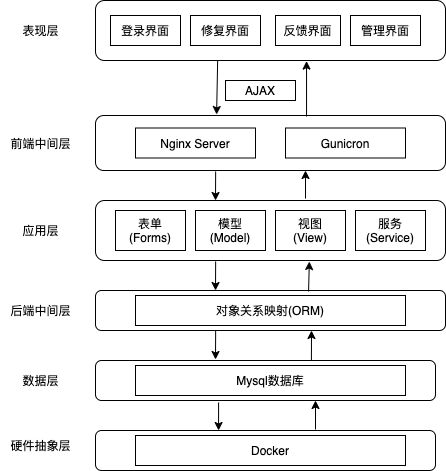
\includegraphics[width=0.7\textwidth]{image/section4/平台架构图.png}
    \captionWithStar{平台架构图}
\end{figure}

\paragraph{表现层}
表现层允许用户通过友好的界面发起任务请求，实现与后端数据处理等模块的交互，并返回结果。

\paragraph{前端中间层}
前端中间层是为了保证平台具有较强的性能，由于所用框架带来的性能缺陷，
本项目通过Nginx与Gunicorn对静态文件与动态请求进行统一管理。
对于静态内容，每次发生改变时，都由Django收集更新的静态，交付Nginx处理；
对于动态内容，则转发到Gunicorn服务器，Gunicorn收到wsgi协议请求后自动解析并回调Django应用。
这样的流程可以让服务器更加安全，性能更有保障。

\paragraph{应用层}
应用层在Django框架的基础上得以实现。通过表单模块实现表单提交验证，通过视图模块定义界面和视图，
通过路由配置模块设定路由跳转，通过模型模块定义数据表以及在信号处理模块中实现语音降噪的数据处理。

\paragraph{后端中间层}
使用框架内的对象关系映射组件给用户提供了完善的数据库接口，
通过便捷的类操作代替繁杂的数据库命令。

\paragraph{数据层}
数据层使用SQLite3作为数据库，可以部署在与Web应用同样的位置，
也可以部署在其它位置，通过远程连接实现访问。
只需简单配置Django Settings就可以实现。

\paragraph{硬件抽象层}
考虑到跨平台部署的便利性，本项目以Docker作为硬件抽象层，通过直接调用硬件资源，
虚拟化出一个Ubuntu20.04操作系统，并在此基础上部署网络服务器以及Django项目。

\clearpage
\subsubsection{模块划分}
在需求分析中，按照功能将平台分为五个模块，数据管理模块、登录注册模块、音频修复模块、意见反馈模块以及项目文档模块。

数据管理模块用来提供便于维护人员管理的后台数据面板；登录注册模块提供访客的身份验证和注册；
音频修复模块提供易操作的音频修复界面；意见反馈模块以邮件的形式提供项目的用户的反馈渠道；
项目文档模块提供本平台的使用指南、核心算法说明以及一系列开发套件的使用方法。
各模块的组成部分如图\ref{平台模块图}所示：
\begin{figure}[htbp]
    \centering
    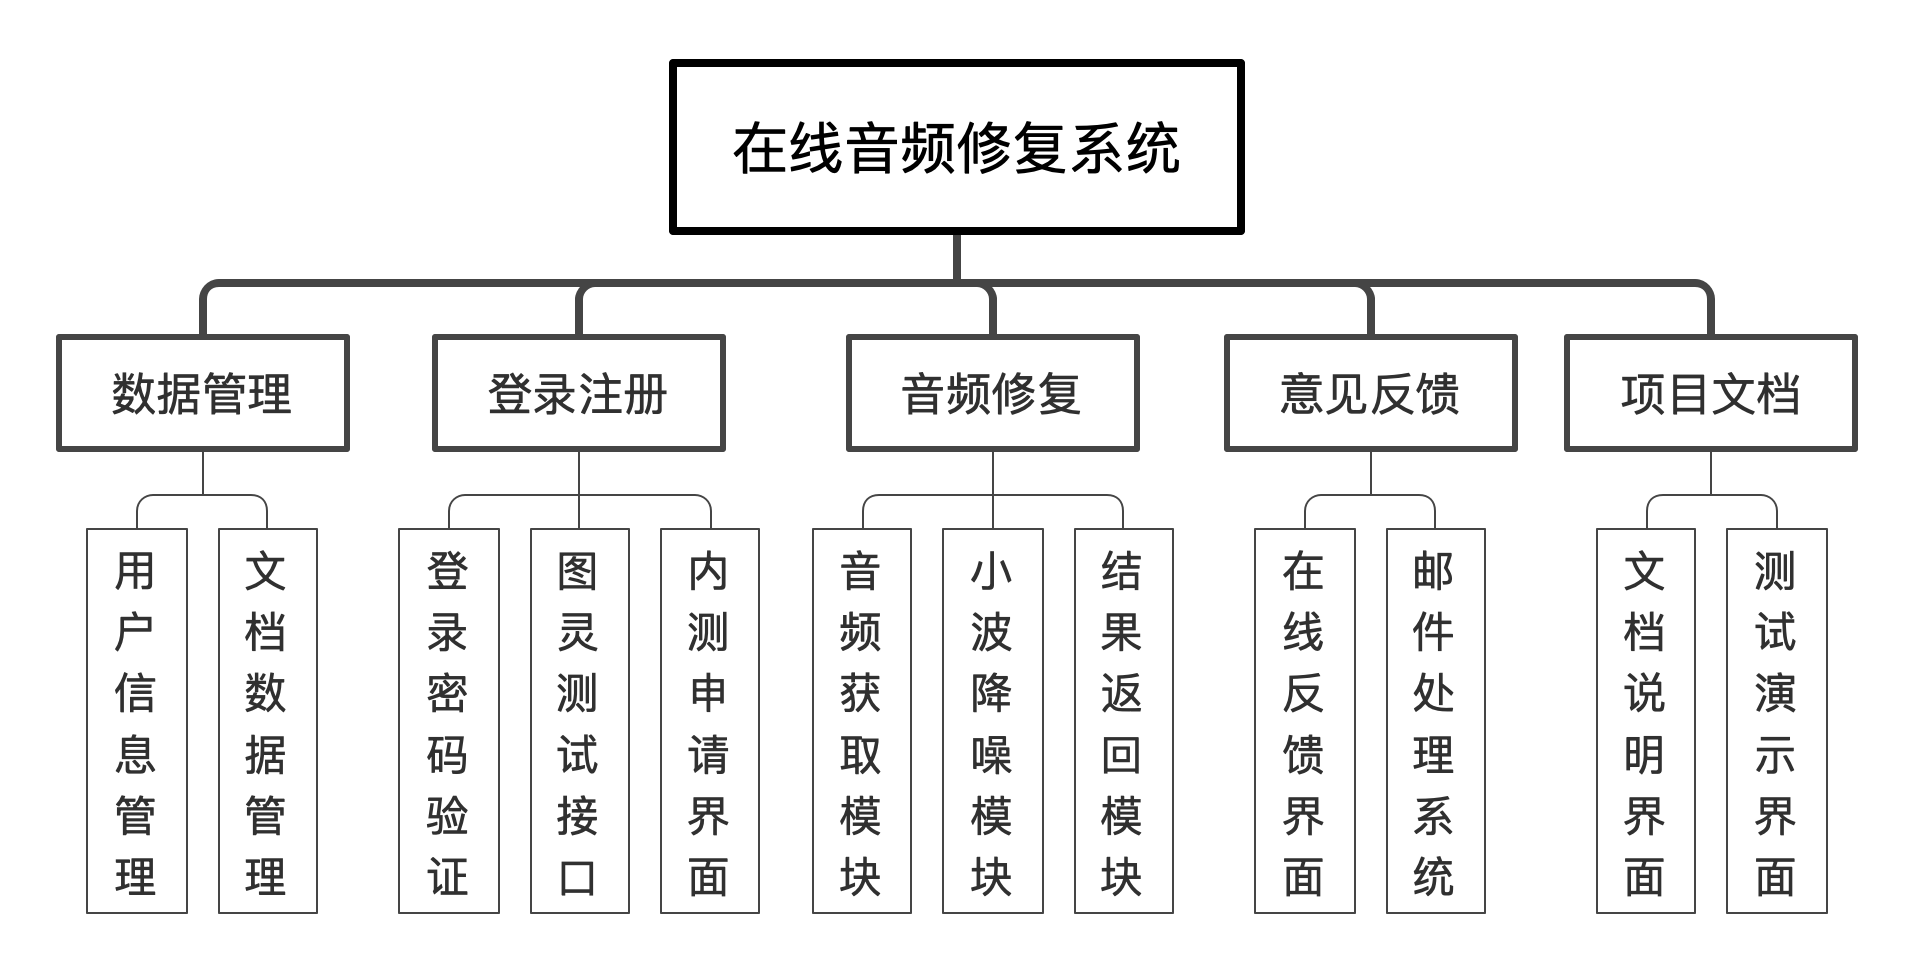
\includegraphics[width=0.85\textwidth]{image/section4/平台模块图.png}
    \captionWithStar{平台模块图}
\end{figure}

\subsubsection{数据库设计}
比起大而全的MySQL而言，SQLite3功能简约，小型化，便于迁移，可靠性好，追求更高的磁盘效率。
考虑本项目中的数据关系较为简单，访问量较小，需要频繁读写磁盘，且核心数据也不适合数据库存储(音频数据库存储不灵活，资源浪费，读写效率查)，
因此本平台选用关系型数据库SQLite3。

因为项目文档模块具有独立性，因此划分出两个数据库，
doc.sqlite3存放文档模块的文章数据，mainsite存放其它数据。
在settings.common中完成数据库的配置后，就可以通过ORM实现数据库的SQL操作。
数据库设计如表\ref{数据库表}所示: 

\begin{table}[ht]
    \centering
    \captionWithStar{数据库表}
    \begin{tabular}{p{2cm}|p{2cm}|p{7cm}}
    \thickhline
    \textbf{库名}               & \textbf{类别}                               & \textbf{表名}                   \\
    \thickhline
    \multirow{13}{*}{mainsite} & \multirow{4}{*}{django}                     & django\_admin\_log            \\
                               &                                             & django\_content\_type         \\
                               &                                             & django\_migrations            \\
                               &                                             & django\_session               \\ \cline{2-3}
                               & \multirow{6}{*}{auth}                       & auth\_group                   \\
                               &                                             & auth\_group\_permissions      \\
                               &                                             & auth\_permission              \\
                               &                                             & auth\_user                    \\
                               &                                             & auth\_user\_groups            \\
                               &                                             & auth\_user\_user\_permissions \\ \cline{2-3}
                               & \multirow{2}{*}{mainsite}                   & profile                       \\
                               &                                             & audio                         \\ \cline{2-3}
                               & sqlite                                      & sequence                      \\
    \thickhline                          
    \multirow{3}{*}{doc}       & django                                      & migrations                    \\ \cline{2-3}
                               & doc                                         & post                          \\ \cline{2-3}
                               & sqlite                                      & sequence                      \\ \cline{2-3}
    \thickhline
    \end{tabular}
\end{table}

Django框架自带的表包含了数据库迁移日志(django\_migrations)、会话数据(session)、系统操作日志(admin\_log)等数据；
Auth模块拥有的表则存储了平台的用户信息(auth\_user)、用户组信息(auth\_group)、用户和用户组的关系(auth\_user\_groups)以及权限和组的关系(auth\_group\_permissions)等。

音频修复模块对应的数据表为profile与audio。
其中，profile继承自auth\_user，实现profile中的user属性与auth\_user的一对一映射，并通过记录使用次数(used\_times)和剩余次数(remaining\_times)更好的管理用户；
audio不绑定profile，而是以公用数据的形式存储，因此只包含文件名(filename)、存储位置(store\_path)、上传时间(upload\_datetime)和尺寸(size)这些音频基础信息。

项目文档模块则只包含post一张表，存储文章的标题(title)、短链接(slug)、正文(body)、摘要(abstract)以及更新时间(pub\_date)。

关键的几个数据表设计如下表所示: 


\begin{table}[ht]
    \centering
    \captionWithStar{audio表}
    \begin{tabular}{p{1cm}p{2.5cm}p{2cm}p{2.5cm}p{3cm}p{2.3cm}}
    \thickhline
    \textbf{序号} & \textbf{字段名}         & \textbf{类型} & \textbf{默认值} & \textbf{属性}          & \textbf{备注} \\
    \thickhline
    1            & id                     & integer      & -              & PRIMARY KEY & 音频 id       \\
    2            & filename               & varchar(255) & test.mp3       &             & 文件名称        \\
    3            & size                   & real         & 0              &             & 文件大小        \\
    4            & upload\_datetime       & datetime     & -              &             & 上传时间        \\
    5            & store\_path            & varchar(255) & /media/audios/ &             & 存储路径        \\
    \thickhline
    \end{tabular}
\end{table}

\begin{table}[ht]
    \centering
    \captionWithStar{user表}
    \begin{tabular}{p{1cm}p{2.5cm}p{2cm}p{2cm}p{3cm}p{2.7cm}}
    \thickhline
    \textbf{序号} & \textbf{字段名}         & \textbf{类型}  & \textbf{默认值}   & \textbf{属性}          & \textbf{备注} \\
    \thickhline
    1            & id                     & integer      & -              & PRIMARY KEY & 用户 id       \\
    2            & password               & varchar(128) & NULL           &             & 密码       \\
    3            & last\_login            & datetime     & -              &             & 上次登录时间        \\
    4            & is\_superuser          & bool         & 0              &             & 是否为超管        \\
    5            & username               & varchar(150) & -              &             & 用户名        \\
    6            & last\_name             & varchar(150) & NULL           &             & 姓氏        \\
    7            & email                  & varchar(254) & NULL           &             & 邮箱        \\
    8            & is\_staff              & bool         & 0              &             & 是否为内部人员        \\
    9            & is\_active             & bool         & 1              &             & 是否活跃        \\
    10           & date\_joined           & datetime     & -              &             & 加入日期        \\
    % 11           & first\_name            & varchar(150) & NULL           &             & 名字        \\
    \thickhline
    \end{tabular}
\end{table}

\begin{table}[ht]
    \centering
    \captionWithStar{profile表}
    \begin{tabular}{p{1cm}p{2.5cm}p{2cm}p{2.5cm}p{3cm}p{2.3cm}}
    \thickhline
    \textbf{序号} & \textbf{字段名}         & \textbf{类型}  & \textbf{默认值}   & \textbf{属性}          & \textbf{备注} \\
    \thickhline
    1            & id                     & integer      & -              & PRIMARY KEY & 档案 id       \\
    2            & used\_times            & integer      & 1000           &             & 使用次数        \\
    3            & remaining\_times       & integer      & 0              &             & 剩余次数        \\
    4            & user\_id               & integer      & -              &             & user映射       \\
    \thickhline
    \end{tabular}
\end{table}

\begin{table}[ht]
    \centering
    \captionWithStar{post表}
    \begin{tabular}{p{1cm}p{2.5cm}p{2cm}p{2.5cm}p{3cm}p{2.3cm}}
    \thickhline
    \textbf{序号} & \textbf{字段名}         & \textbf{类型}  & \textbf{默认值}   & 属性          & \textbf{备注} \\
    \thickhline
    1            & id                     & integer      & -              & PRIMARY KEY & 文章 id       \\
    2            & title                  & varchar(200) & -              &             & 文章名称        \\
    3            & slug                   & varchar(200) & -              &             & 短链接        \\
    4            & body                   & text         & NULL           &             & 正文        \\
    5            & pub\_date              & datetime     & -              &             & 更新时间       \\
    6            & abstract               & text         & NULL           &             & 摘要        \\
    \thickhline
    \end{tabular}
\end{table}

\clearpage
\subsection{平台具体实现}
本节在完成项目需求和明确概要设计的基础上，简要叙述开发测试环境的创建与各模块的实现方式。

\subsubsection{开发测试环境搭建}
考虑到项目最终要部署到谷歌云上的虚拟机实例，在本地已经使用类Unix系统作为开发环境的情况下，仍需要搭建符合最终部署环境需求的本地测试环境。
最终选用由Canonical开发的Multipass下的Ubuntu20.04环境作为本地测试环境。
\begin{figure}[htbp]
    \centering
    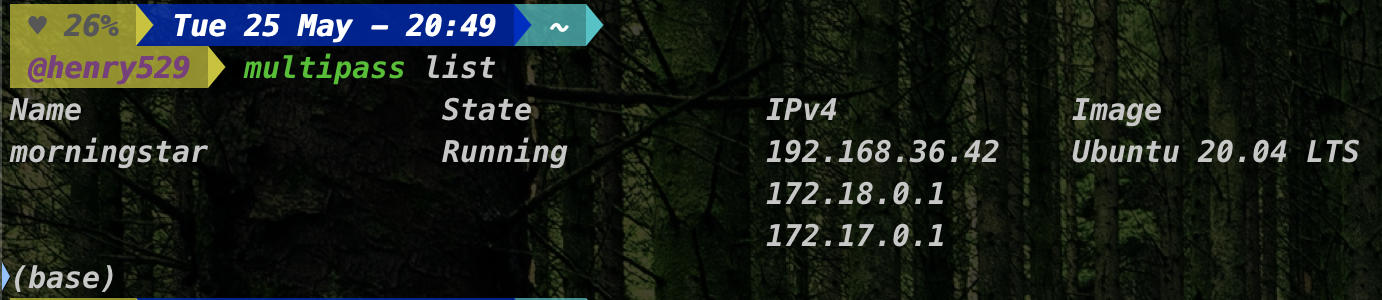
\includegraphics[width=0.7\textwidth]{image/section4/multipass.png}
    \captionWithStar{本地Multipass测试环境}
\end{figure}


开发过程中使用到的框架、组件和第三方库信息如表\ref{所用框架、组件、库信息表}所示: 

\begin{table}[htbp]
    \centering
    \captionWithStar{所用框架、组件、库信息表}
    \begin{tabular}{cr@{.}ll}
    \hline
    \textbf{框架、组件、库}          & \multicolumn{2}{c}{\textbf{版本}} & \textbf{备注}                \\
    \hline
    \textit{requests}                  & 2 & 25         & HTTP库，实现请求发送             \\
    \textit{django}                     & 3 & 2         & 基础的Web框架                   \\
    \textit{django-recaptcha}           & 2 & 0         & 实现登录界面上的Google Recaptcha验证 \\
    \textit{mysqlclient}                & 2 & 0         & 用于连接数据库                    \\
    \textit{Bootstrap}                  & 5 & 0         & 前端框架                      \\
    \textit{django-markdown-deux}       & 1 & 0         & 提供文档markdown支持             \\
    \textit{django-user-agents}         & 2 & 2         & 配合前端适配不同的终端                \\
    \textit{jupyterlab}                 & 3 & 0         & 算法测试环境                     \\
    \textit{pywavelets}                 & 1 & 1         & 基于numpy的第三方小波库             \\
    \textit{pydub}                      & 0 & 25        & 支持基础的音频读写查操作               \\
    \textit{selenium}                   & 3 & 141       & 用于机器人自动化测试                \\
    \textit{gunicorn}                   & 20& 1         & WSGI http服务器               \\
    \textit{gcloud}                     & 342 & 0       & Google Cloud SDK 命令行工具   \\
    \textit{pipenv}                     & 2020 & 11     & 虚拟python运行环境与包管理      \\ 
    \hline
    \end{tabular}
\end{table}

\subsubsection{数据管理模块实现}
数据管理模块主要提供核心数据面板以及项目运维面板。
其中，核心数据面板提供诸如用户信息、文章信息等项目直接相关的数据的管理，
而项目运维面板则提供Docker、Web服务器等部署相关的功能管理。

\paragraph{核心数据面板}
因为所用框架自带后台管理系统和用户验证功能，所以只需对其稀疏封装，
就可以实现自定义的核心数据面板。
在实现模型检查与数据库迁移后，就可以使用超管账号登录核心数据面板。
效果如图\ref{核心数据面板}所示：

\begin{figure}[htbp]
    \centering
    \begin{minipage}[t]{0.46\textwidth}
        \centering
        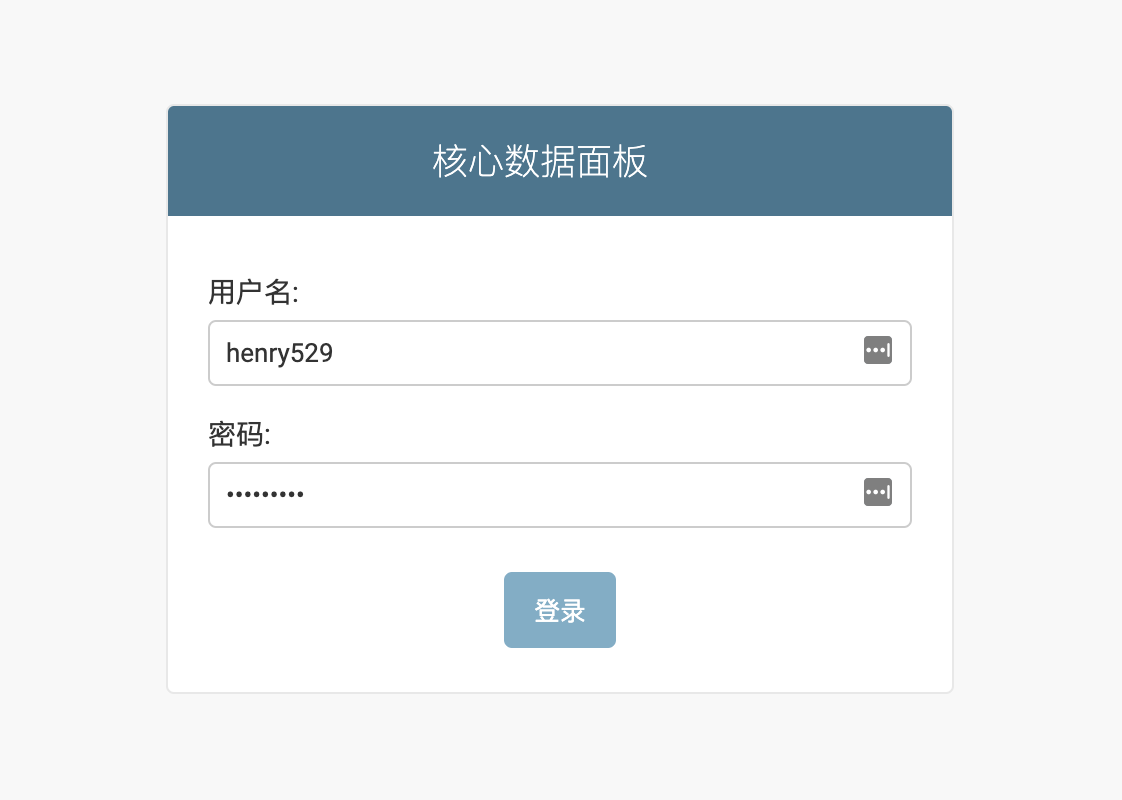
\includegraphics[width=\linewidth , height=0.6\linewidth]{image/section4/admin-login.png}
    \end{minipage}
    \begin{minipage}[t]{0.46\textwidth}
        \centering
        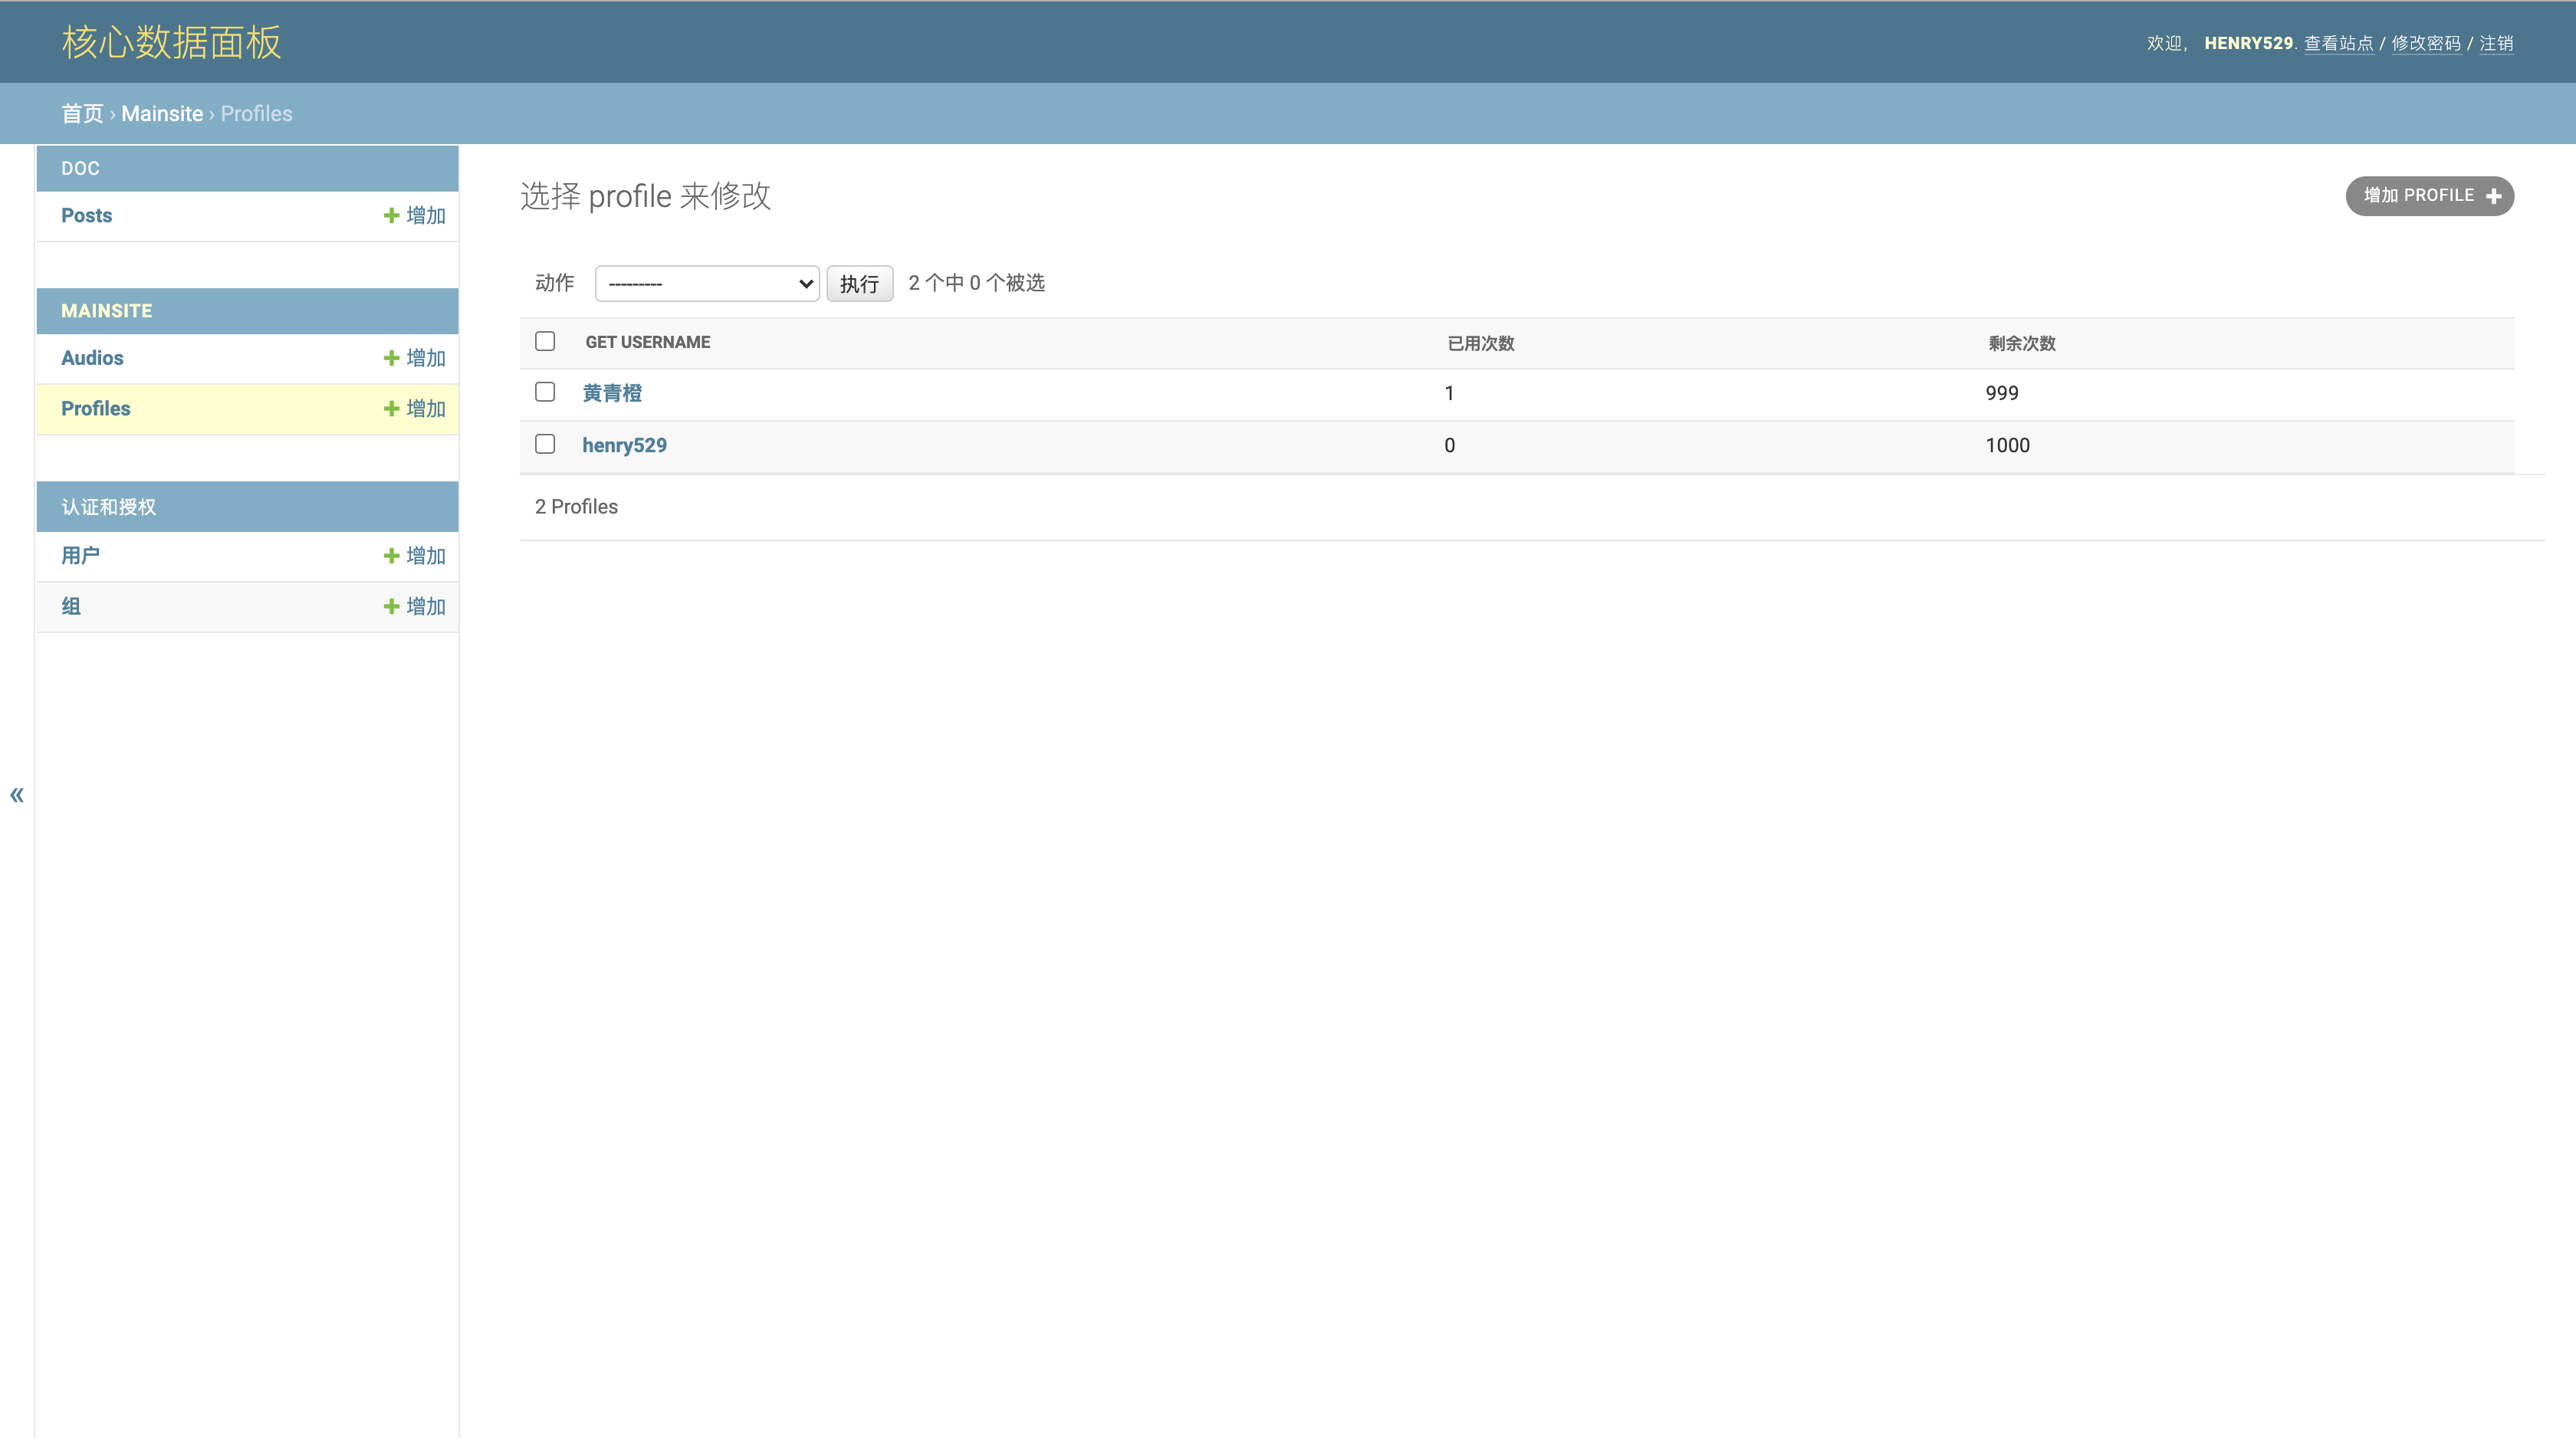
\includegraphics[width=\linewidth , height=0.6\linewidth]{image/section4/admin.png}
    \end{minipage}
    \captionWithStar{核心数据面板}
\end{figure}

\paragraph{项目运维面板}
考虑到本项目的参与者可能专精信号处理，未必熟悉网站运维，因此一个可视化的运维面板必不可少。
本项目的运维面板通过宝塔面板来实现，效果如图\ref{项目运维面板}所示: 
\begin{figure}[htb]
    \centering
    \begin{minipage}[t]{0.46\textwidth}
        \centering
        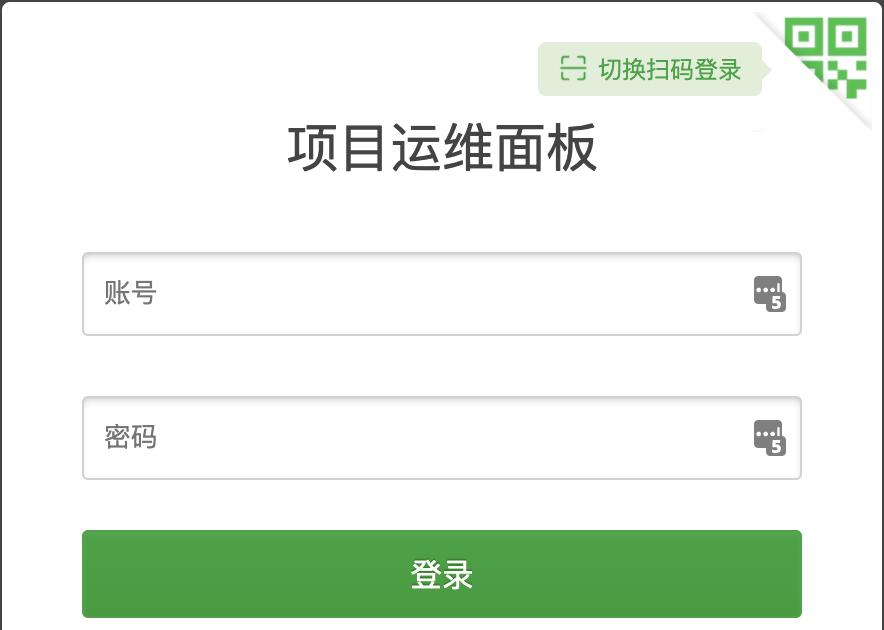
\includegraphics[width=\linewidth , height=0.6\linewidth]{image/section4/bt-login.png}
    \end{minipage}
    \begin{minipage}[t]{0.46\textwidth}
        \centering
        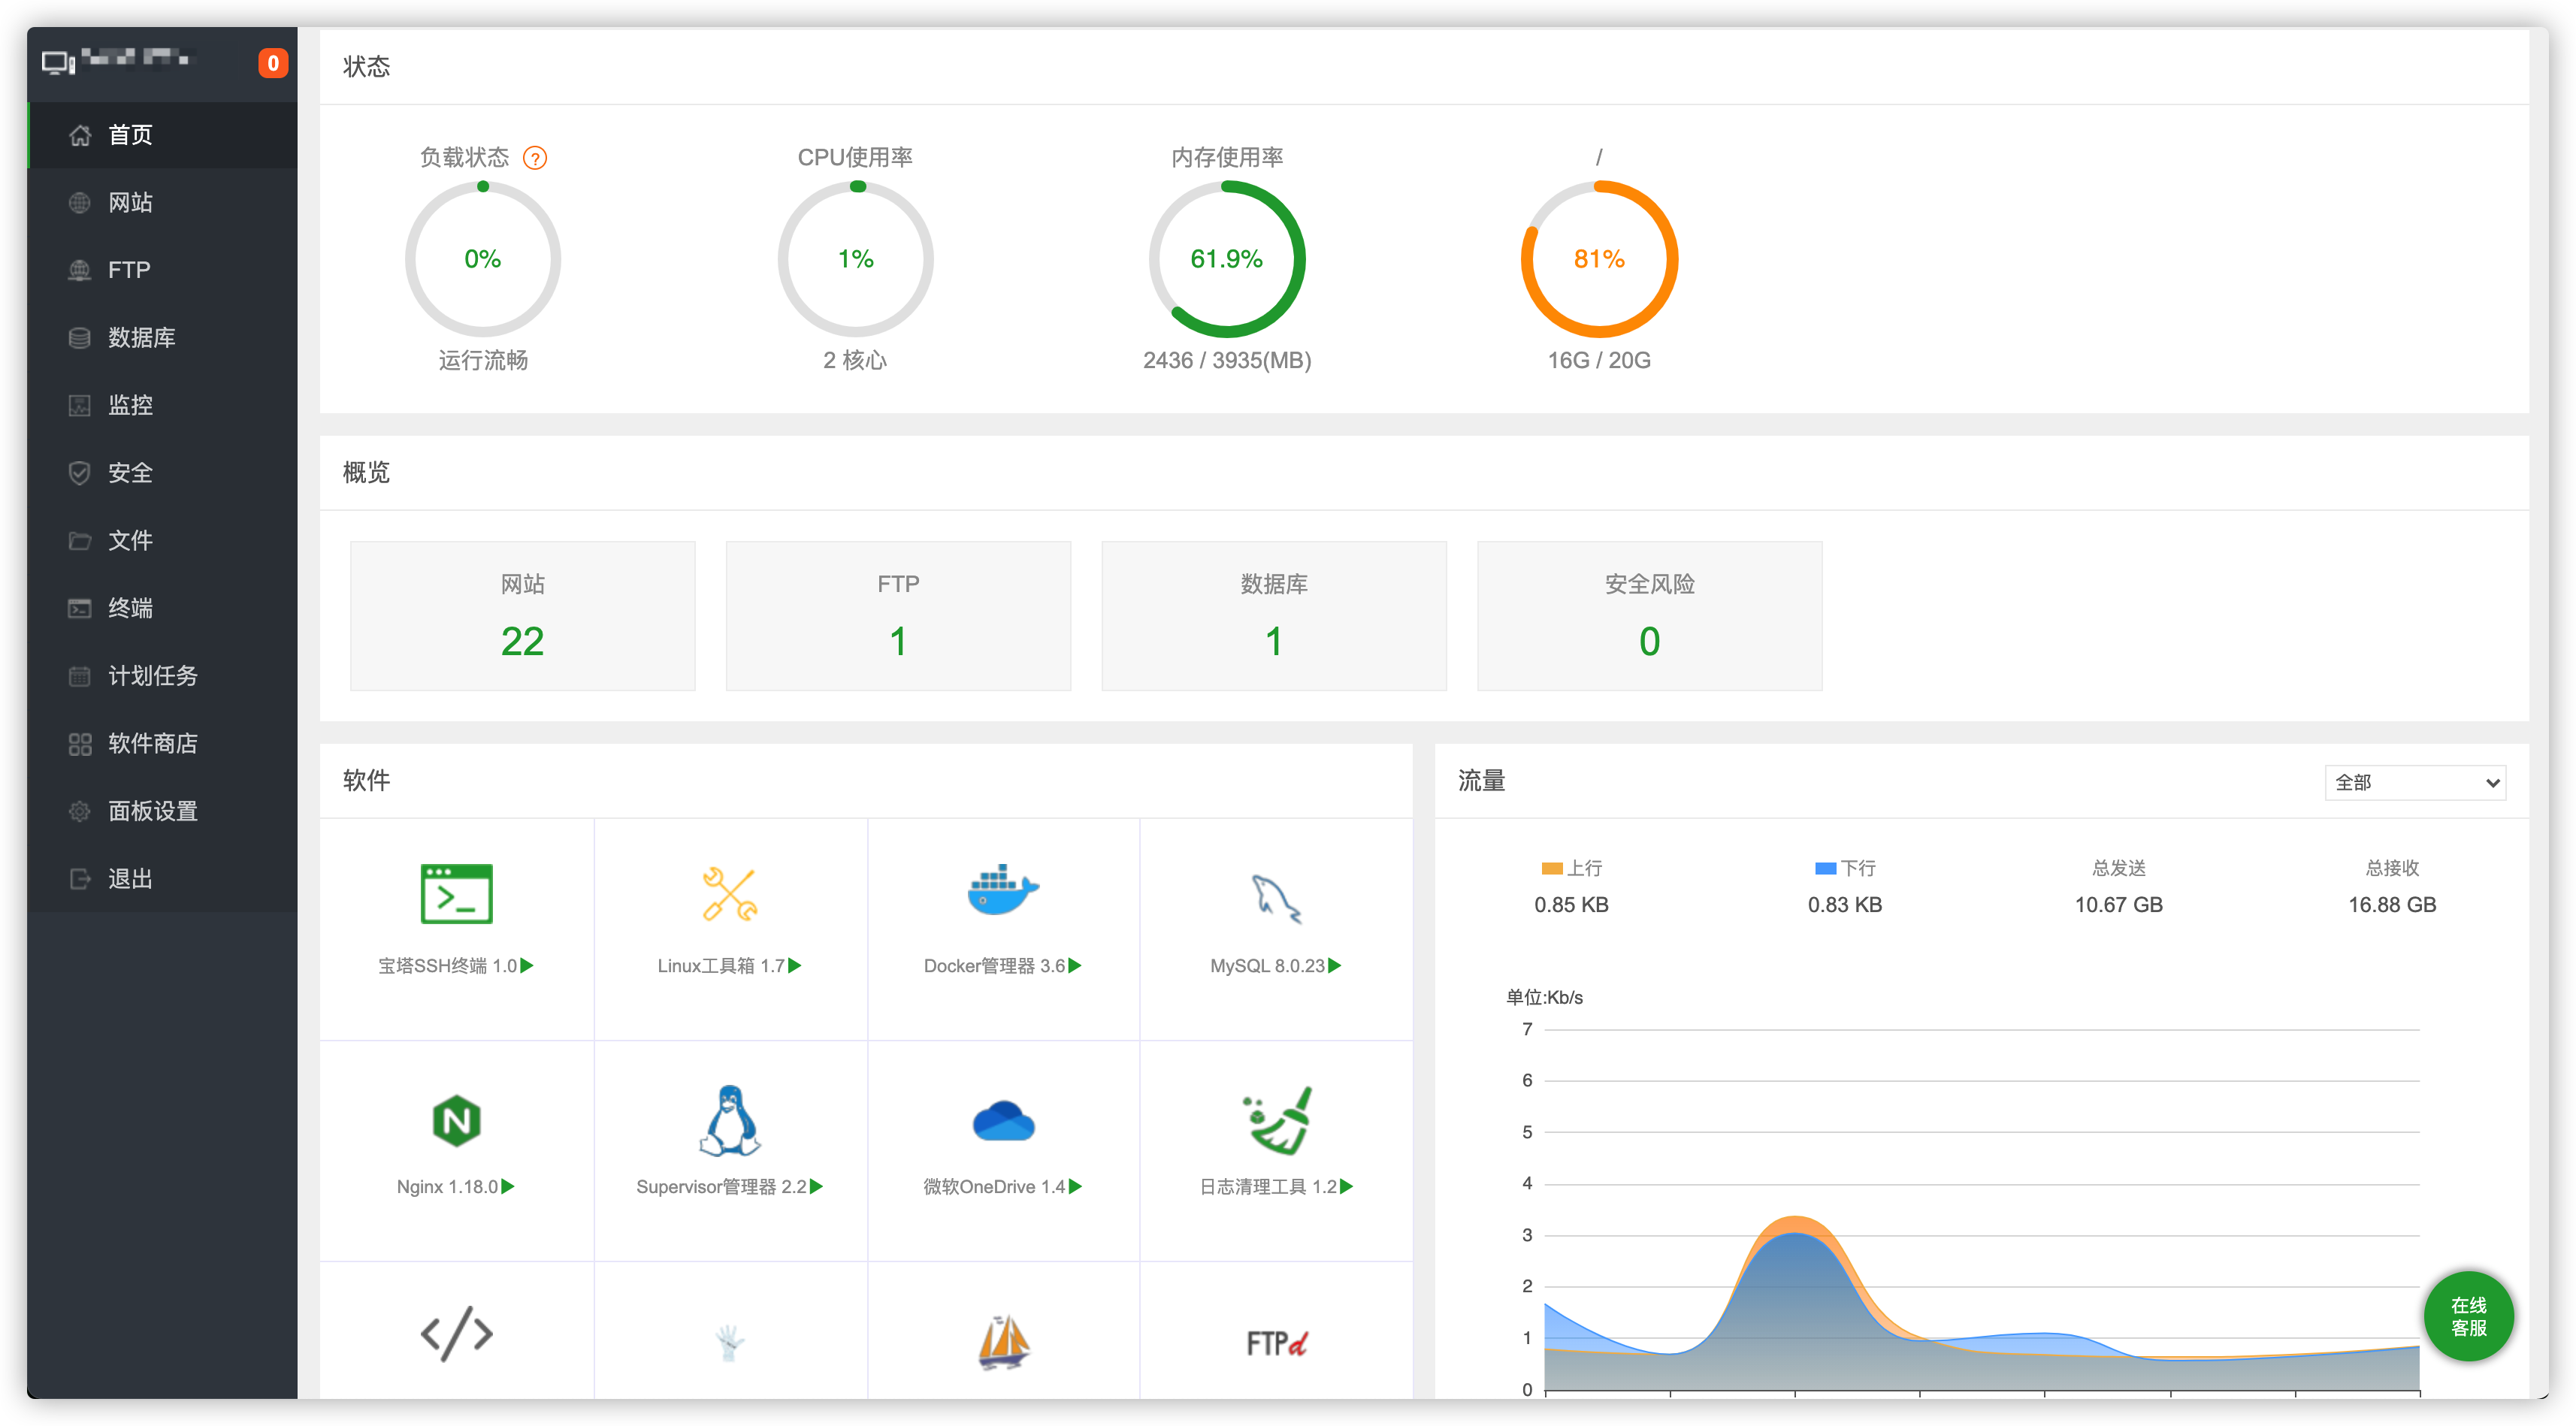
\includegraphics[width=\linewidth , height=0.6\linewidth]{image/section4/bt.png}
    \end{minipage}
    \captionWithStar{项目运维面板}
\end{figure}


\subsubsection{登录注册模块实现}

\paragraph{界面设计}

登录注册界面的前端由Bootstrap实现，如图\ref{登录注册界面}所示。
考虑到项目仍处于内测阶段，因此只在登录界面上开辟小板块，引导访客使用邮件做注册申请，后台会通过正则匹配，获取包含“注册”
的邮件，并转发至管理员信箱，等待进一步处理。

\begin{figure}[htbp]
    \centering
    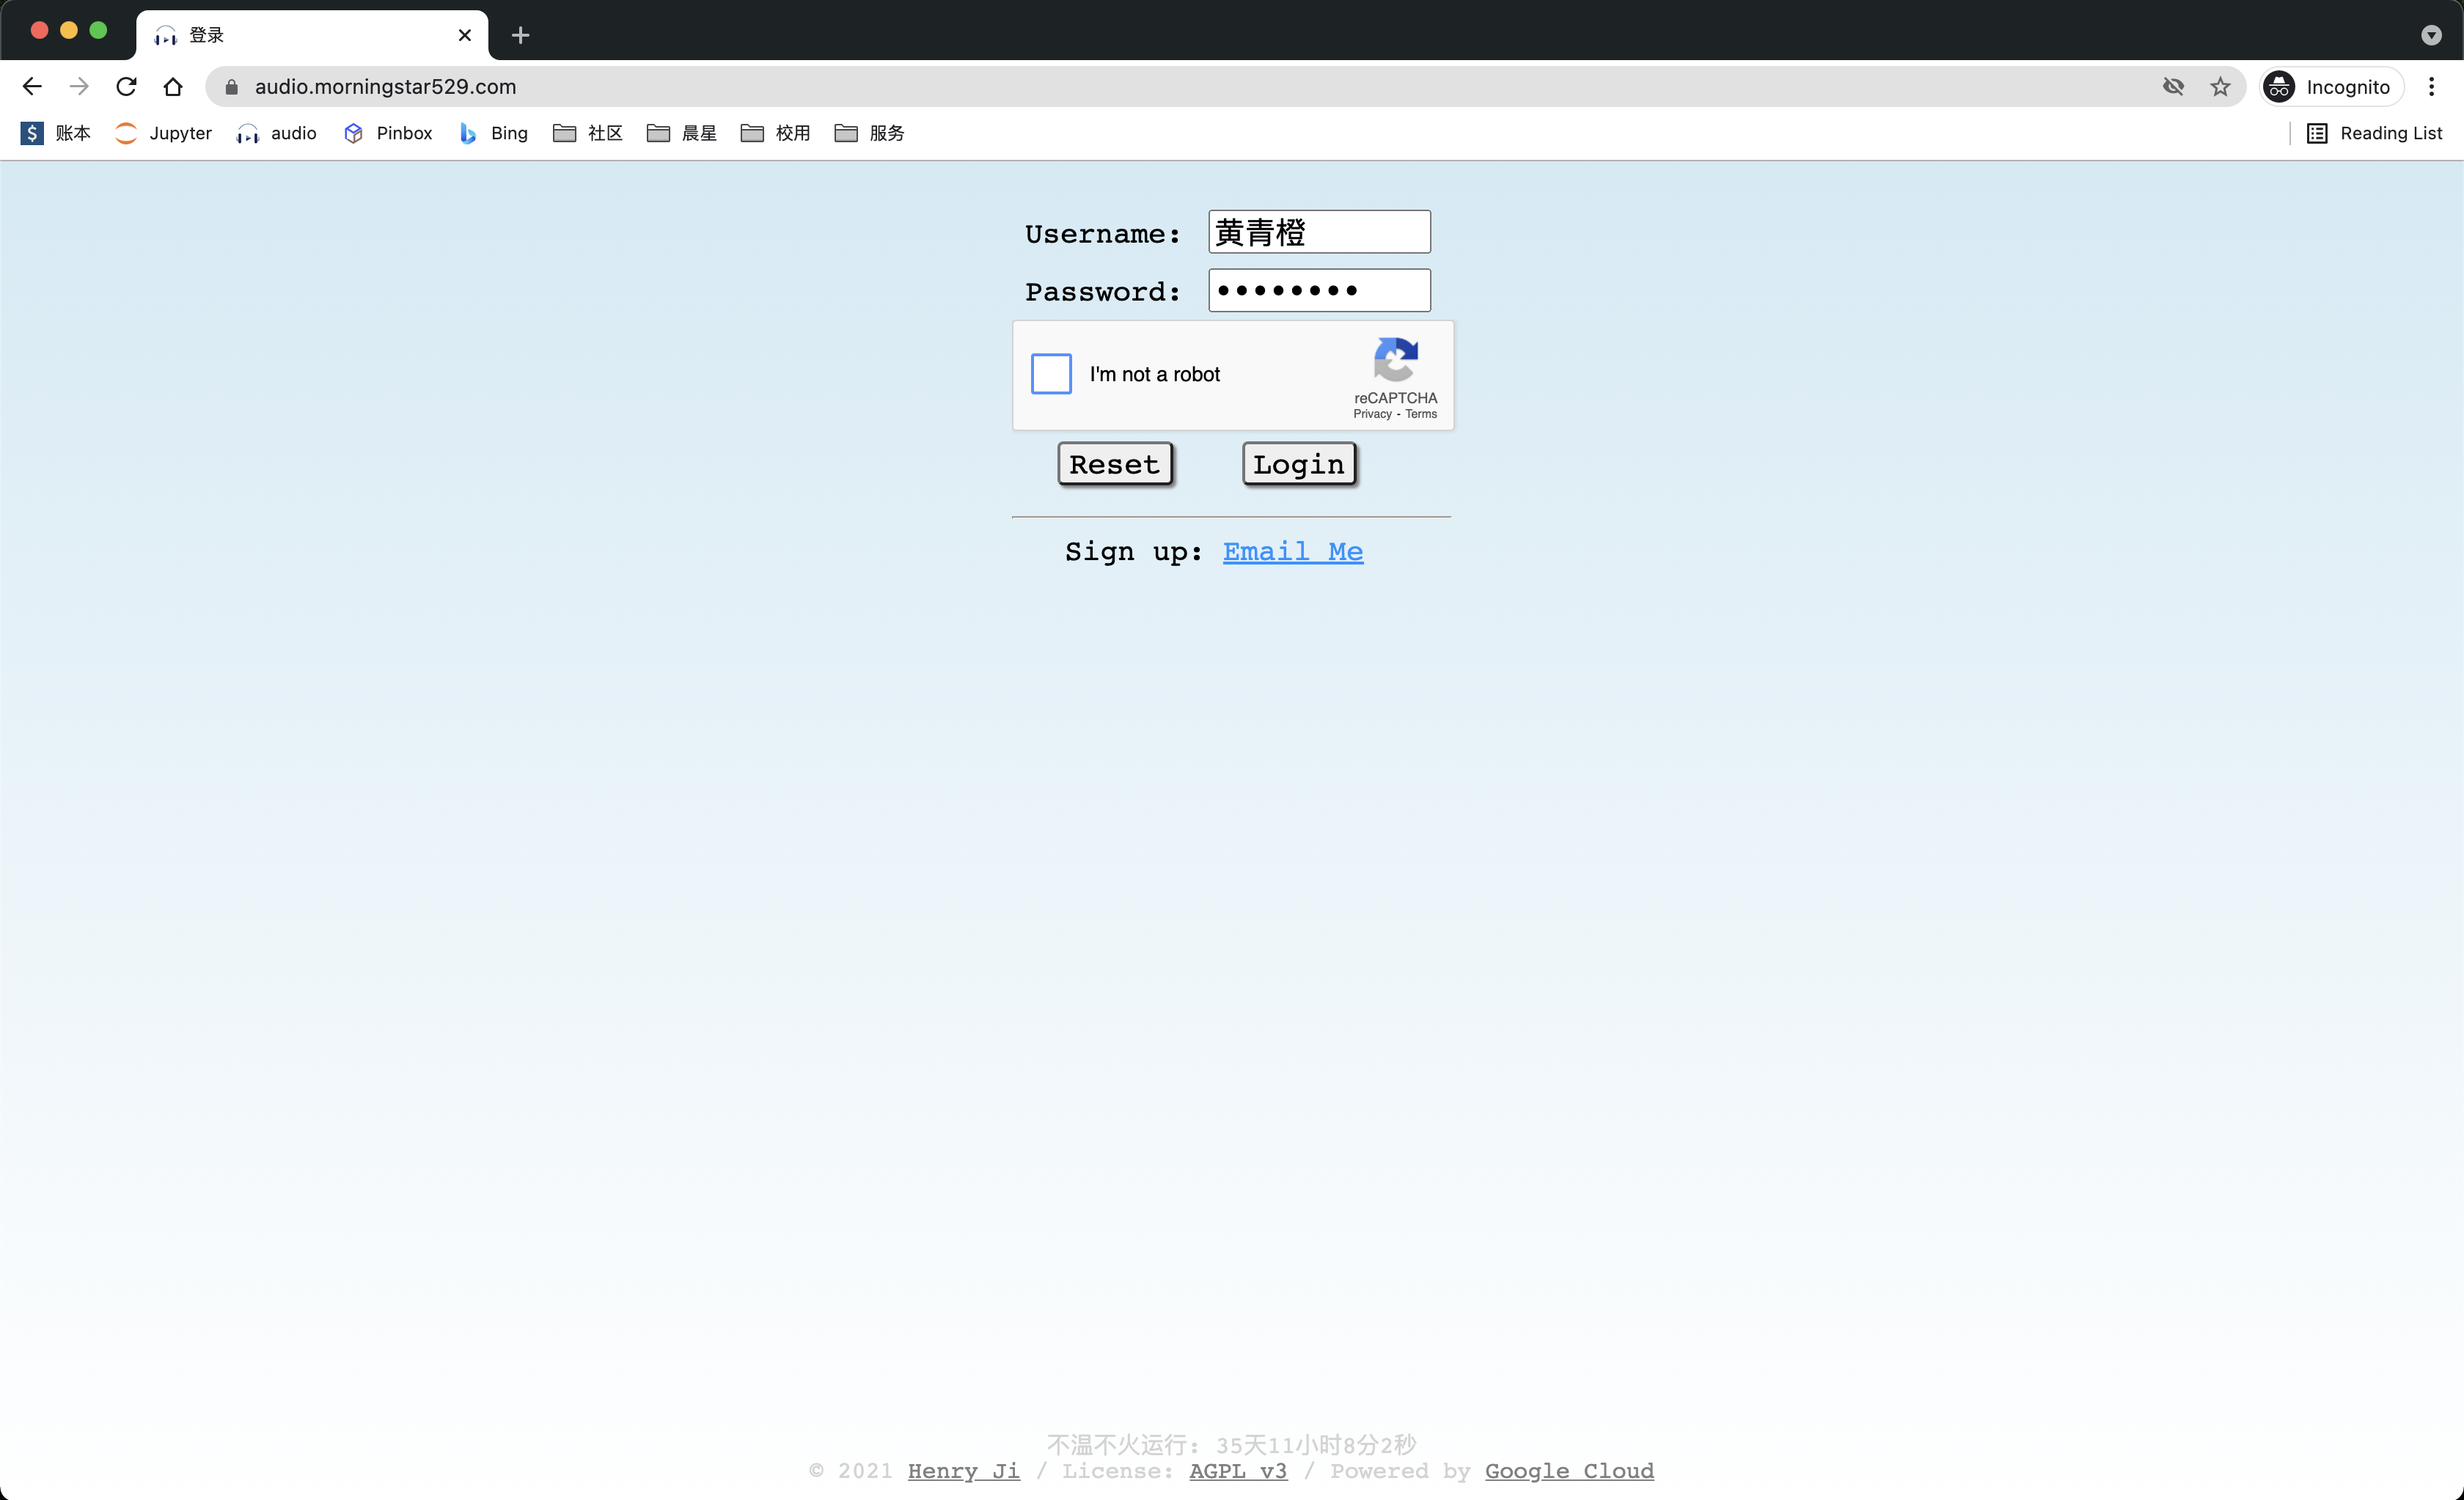
\includegraphics[width=1\textwidth]{image/section4/login.png}
    \captionWithStar{登录注册界面}
\end{figure}

\paragraph{交互逻辑}

在用户填写完username和password后，还需要通过Google Recaptcha V2的图灵测试。
(出于到用户友好的考量，已将难度调到最低，对流量攻击已有较好的抵御能力)
图灵验证通过后，就能以LoginForm表单的形式提交表单。
后端收到请求后，先用表单类的valid方法进行验证诸如长短、数据类型等的格式是否正确，
之后使用user的authenticate方法验证用户名和密码是否正确。
顺利通过后就保存账号信息到session并返回主页，否则重定向到登录界面。


\subsubsection{音频修复模块实现}
\paragraph{界面设计}
音频修复模块的界面使用经典的圣杯布局，效果如图\ref{音频修复界面}所示:

\begin{figure}[htbp]
    \centering
    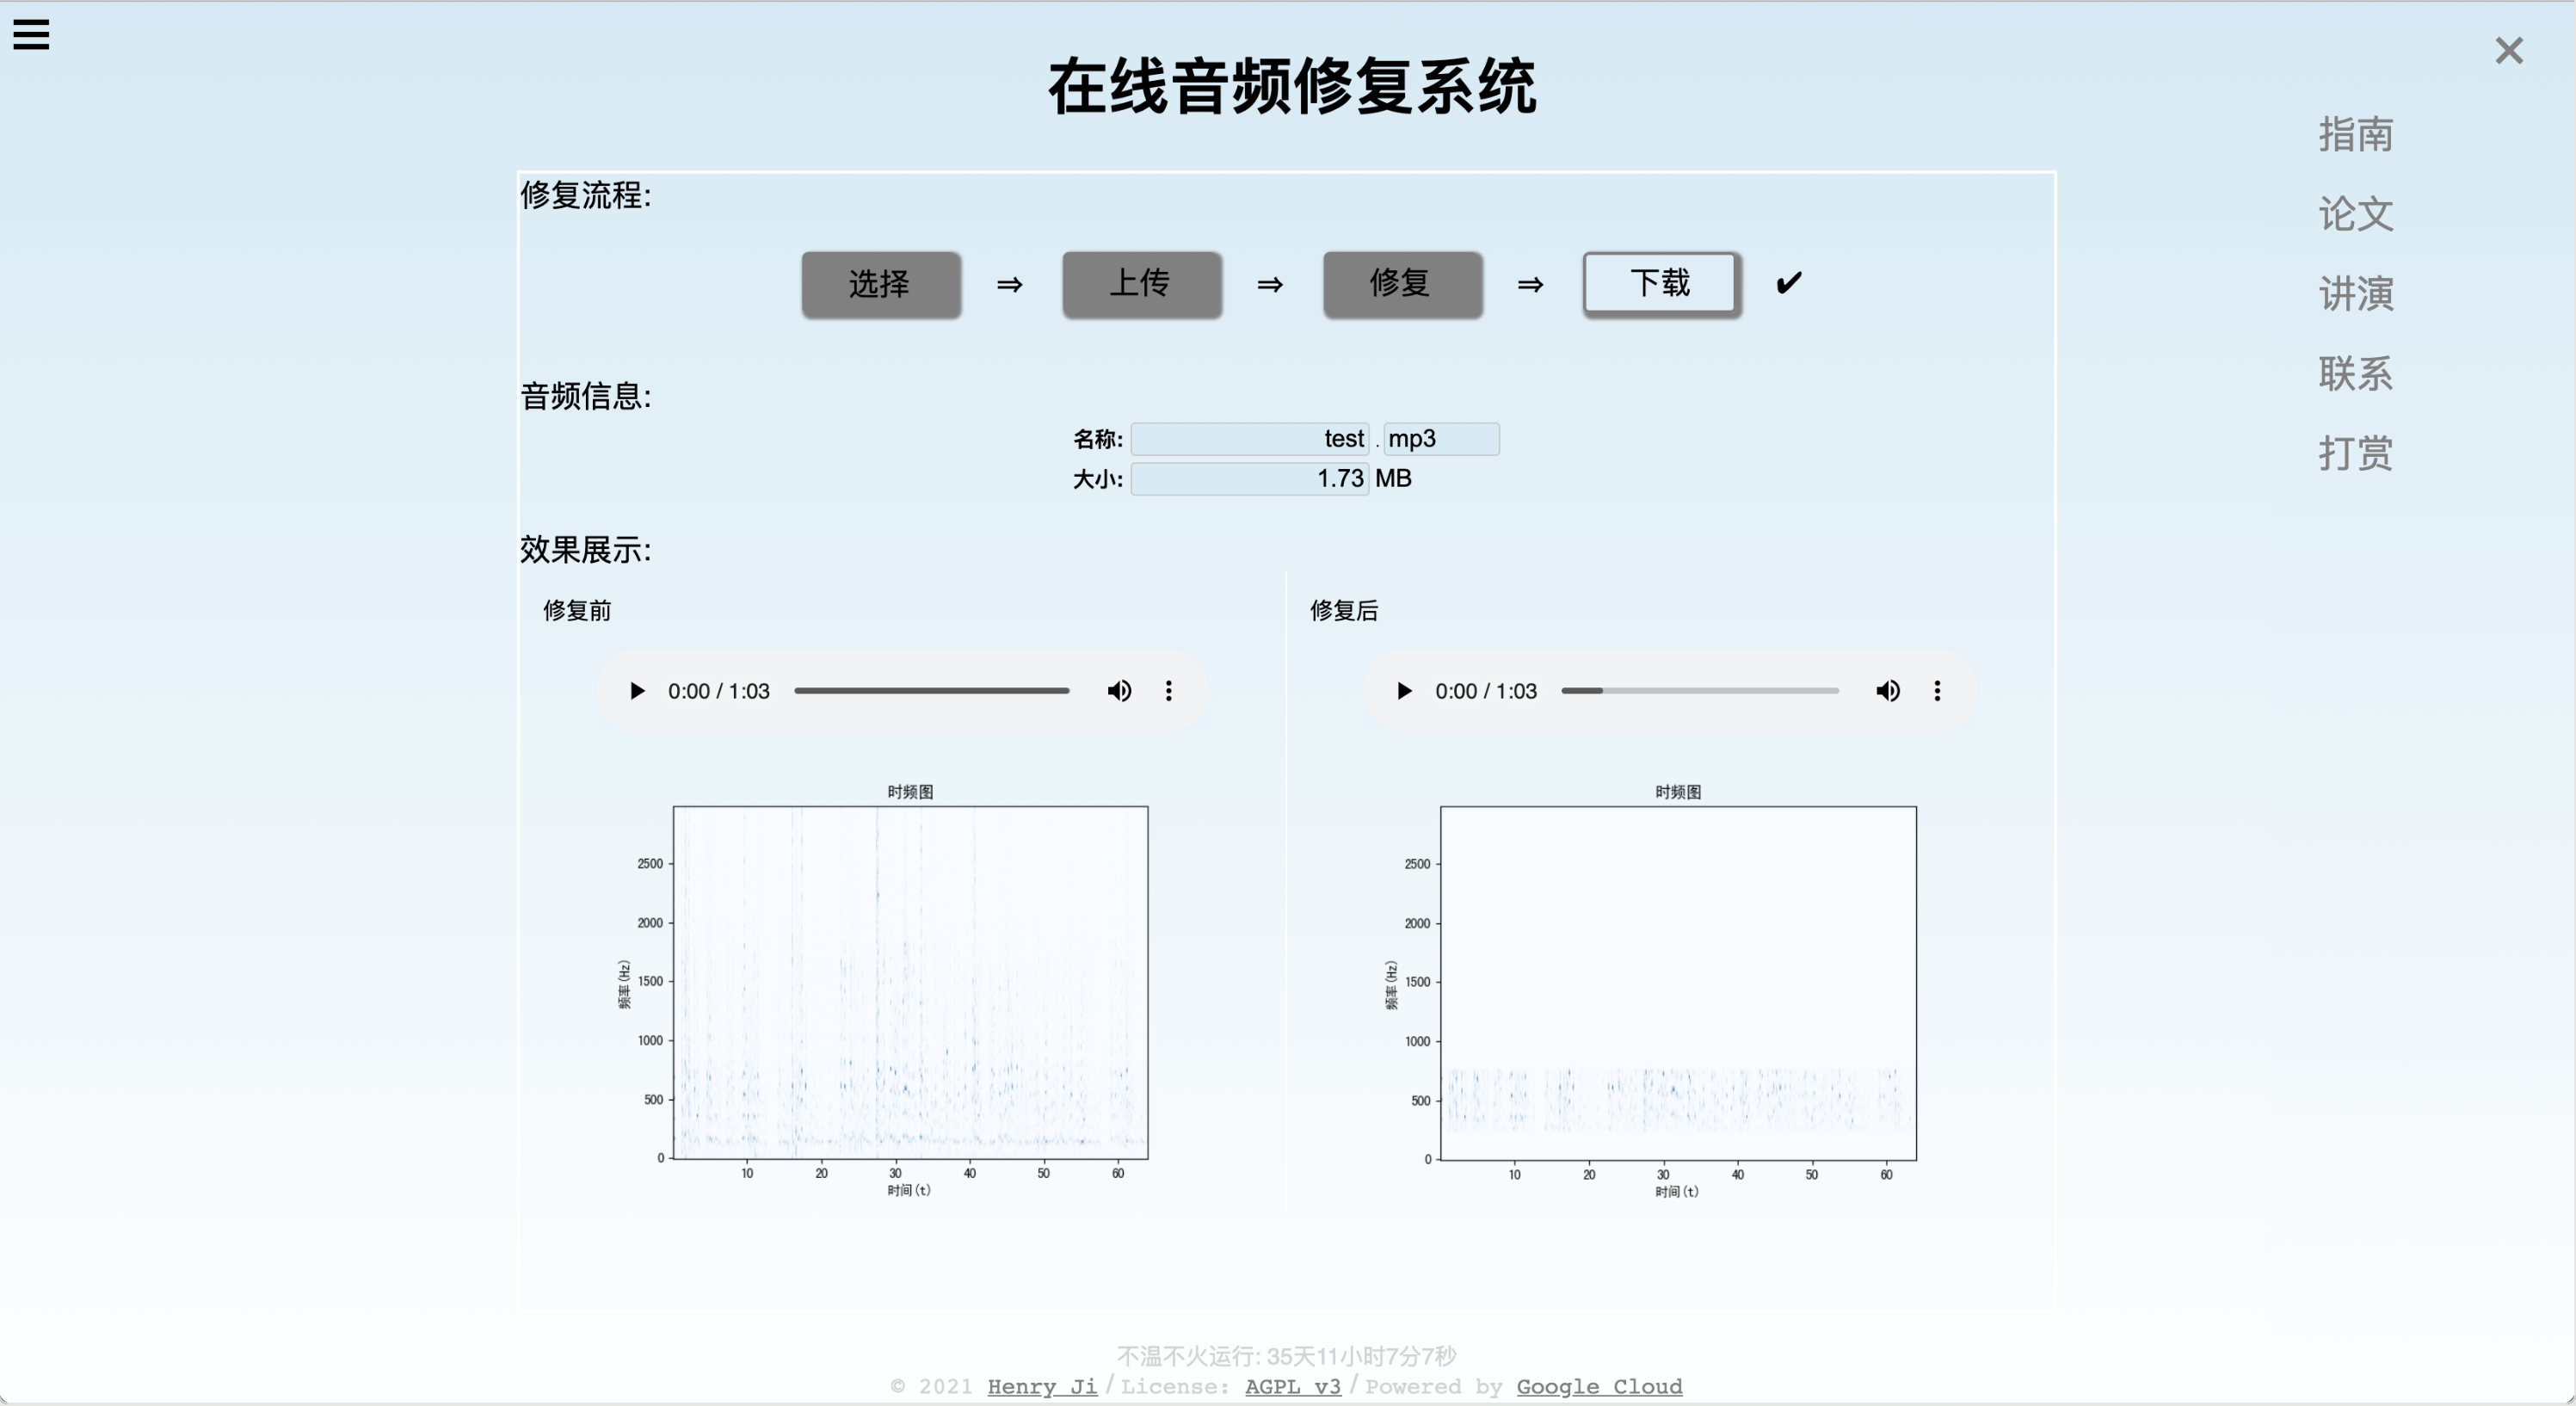
\includegraphics[width=1\textwidth]{image/section4/main.png}
    \captionWithStar{音频修复界面}
\end{figure}

\begin{enumerate}[a)]
    \item 为保持界面整洁，页面上只显示“修复流程”、“音频信息”、“效果演示”三个版块，其余信息都通过侧边栏的外链给出。
    \item 为了实现更好的交互，本模块严格按照SPA的规则，所有的HTTP请求都是通过AJAX的形式发出。
    \item 为了提高鲁棒性，只有当用户按照箭头指向挨个点击时，按键才会显现，避免了误操作；
    通过箭头指向还使得操作逻辑更加友好。
    \item 选用圣杯布局，在不同的终端上都有较好的展示效果。
\end{enumerate}

\paragraph{交互逻辑}
音频修复流程的逻辑如图\ref{音频修复流程}所示: 
\begin{figure}[htbp]
    \centering
    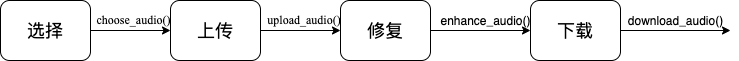
\includegraphics[width=\textwidth]{image/section4/音频修复流程.png}
    \captionWithStar{音频修复流程}
\end{figure}

\begin{enumerate}
\item \emph{选择}：登录完成后进入本界面，点击“选择”按钮或快捷键"Shift+C"触发文件选择对话框并灰化“选择”按钮；
选择好文件后，前端的js脚本检测到file标签中的数值发生变动，触发choose\_audio()方法，自动获取文件名、扩展名
以及文件大小，并生成对应的存储位置、时间戳；显示一系列音频信息到页面对应区域，同时显示出“上传”按钮。
\item \emph{上传}：点击“上传”按钮或快捷键"Shift+U"触发upload\_audio()方法，灰化“上传”按钮，构建FormData，将音频文件名、扩展名、文件大小、存储路径、时间戳以及文件本身打包，以POST请求的方式通过AJAX发往后端的/upload\_api；
后端接收到这一request后，从POST请求中拆分出对应数据并用session记录，以文件名、文件大小和存储位置构建出新的audio对象，通过ORM存入数据库；完成后刷新主界面并显示修复按钮。
\item \emph{修复}：点击“修复”按钮或快捷键"Shift+R"触发enhance\_audio()方法，灰化“修复”按钮，通过AJAX发送待修复音频存储位置至/enhance\_api，并显示出进度条；
后端解析这一请求后，获取存储位置后开始音频增强处理；修复完成后返回修复后音频的存储位置，刷新主界面并显示下载按钮。
\item \emph{下载}：点击“下载”按钮或快捷键"Shift+D"触发download\_audio()方法，灰化“修复”按钮，下载新音频到浏览器默认下载位置；
清空除去username和password以外所有的session数据，然后刷新界面。

\end{enumerate}

\subsubsection{意见反馈模块实现}

\paragraph{界面设计}
此界面启发自小甲鱼的邮箱，使用简易的局中布局，效果如图\ref{意见反馈界面}所示: 

\begin{figure}[htbp]
    \centering
    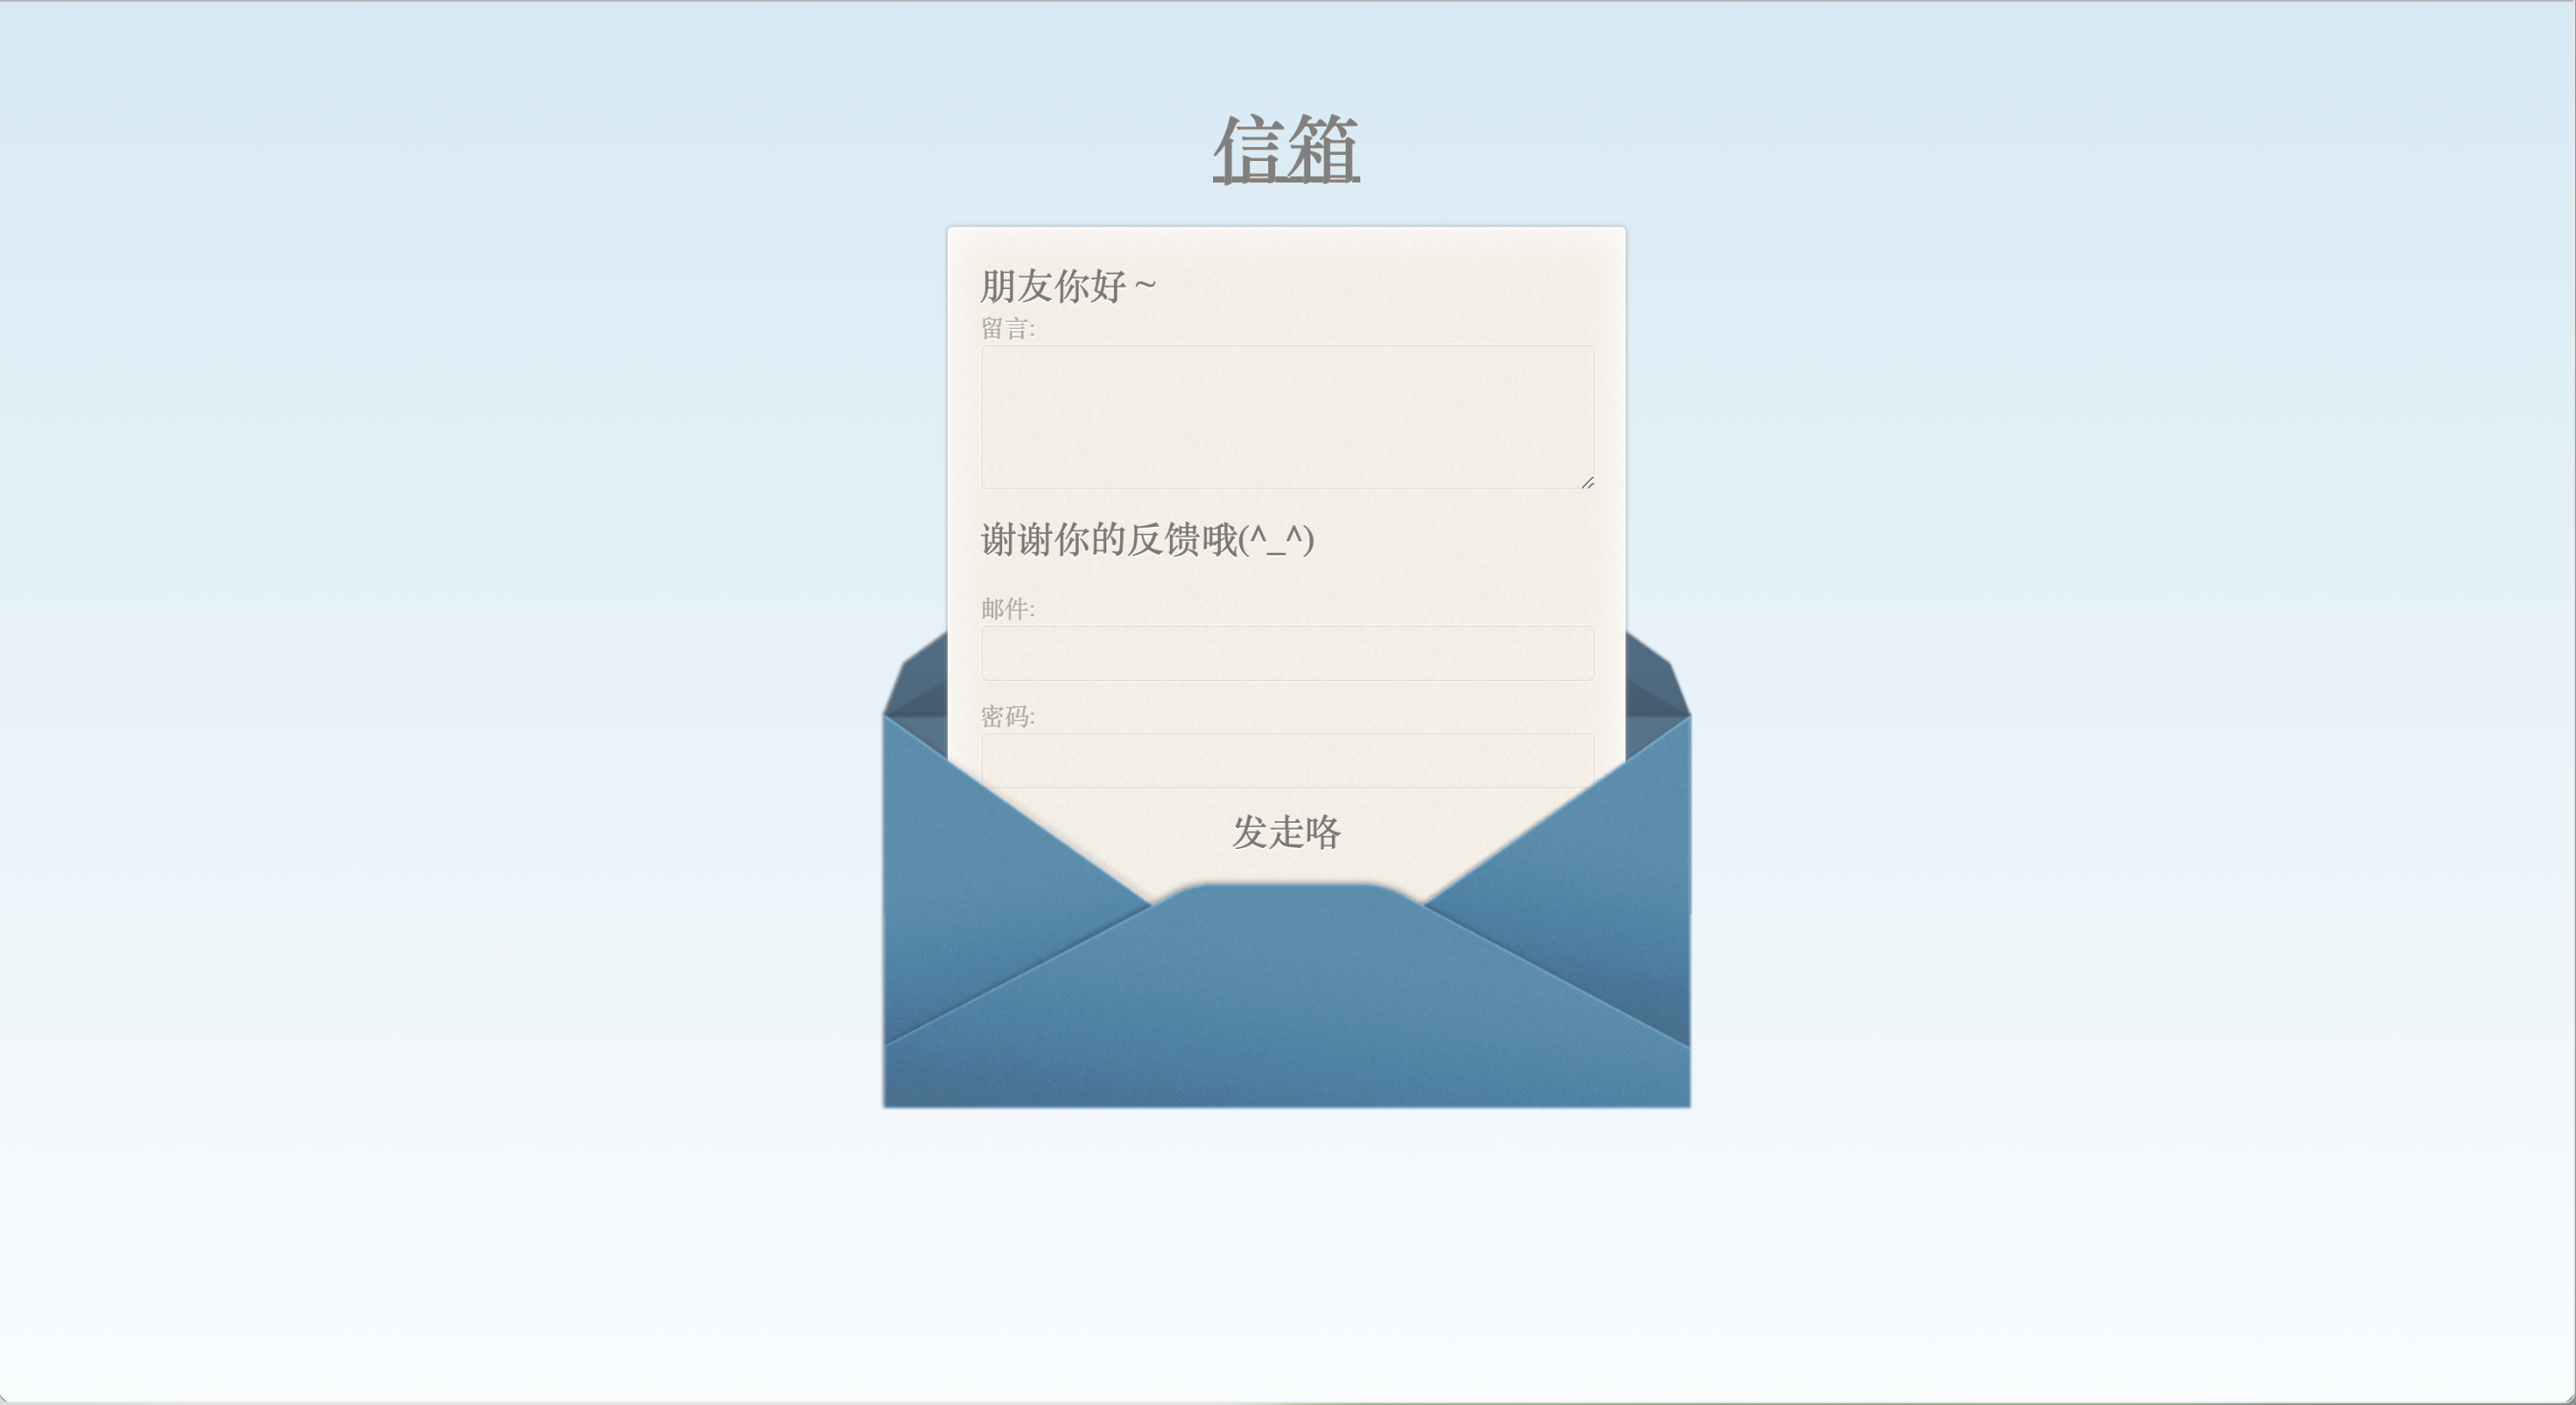
\includegraphics[width=0.7\textwidth]{image/section4/email.png}
    \captionWithStar{意见反馈界面}
\end{figure}


\paragraph{后端实现}
通过第三方邮箱库，实现邮件的发送接收功能；
一旦接收到访客发送的邮件，就将其保存到数据库，而后通过正则表达式，根据邮件的主题将邮件分成三类：注册申请、bug反馈和其它；
根据不同类型的邮件重新调整格式，推送到管理员邮箱。


\newpage
\subsubsection{项目文档模块实现}
\paragraph{界面设计}
此模块的界面基于Bootstap网格系统设计而成，以2:10划分侧边栏与正文。
效果如图\ref{项目文档界面}所示:

\begin{figure}[htbp]
    \centering
    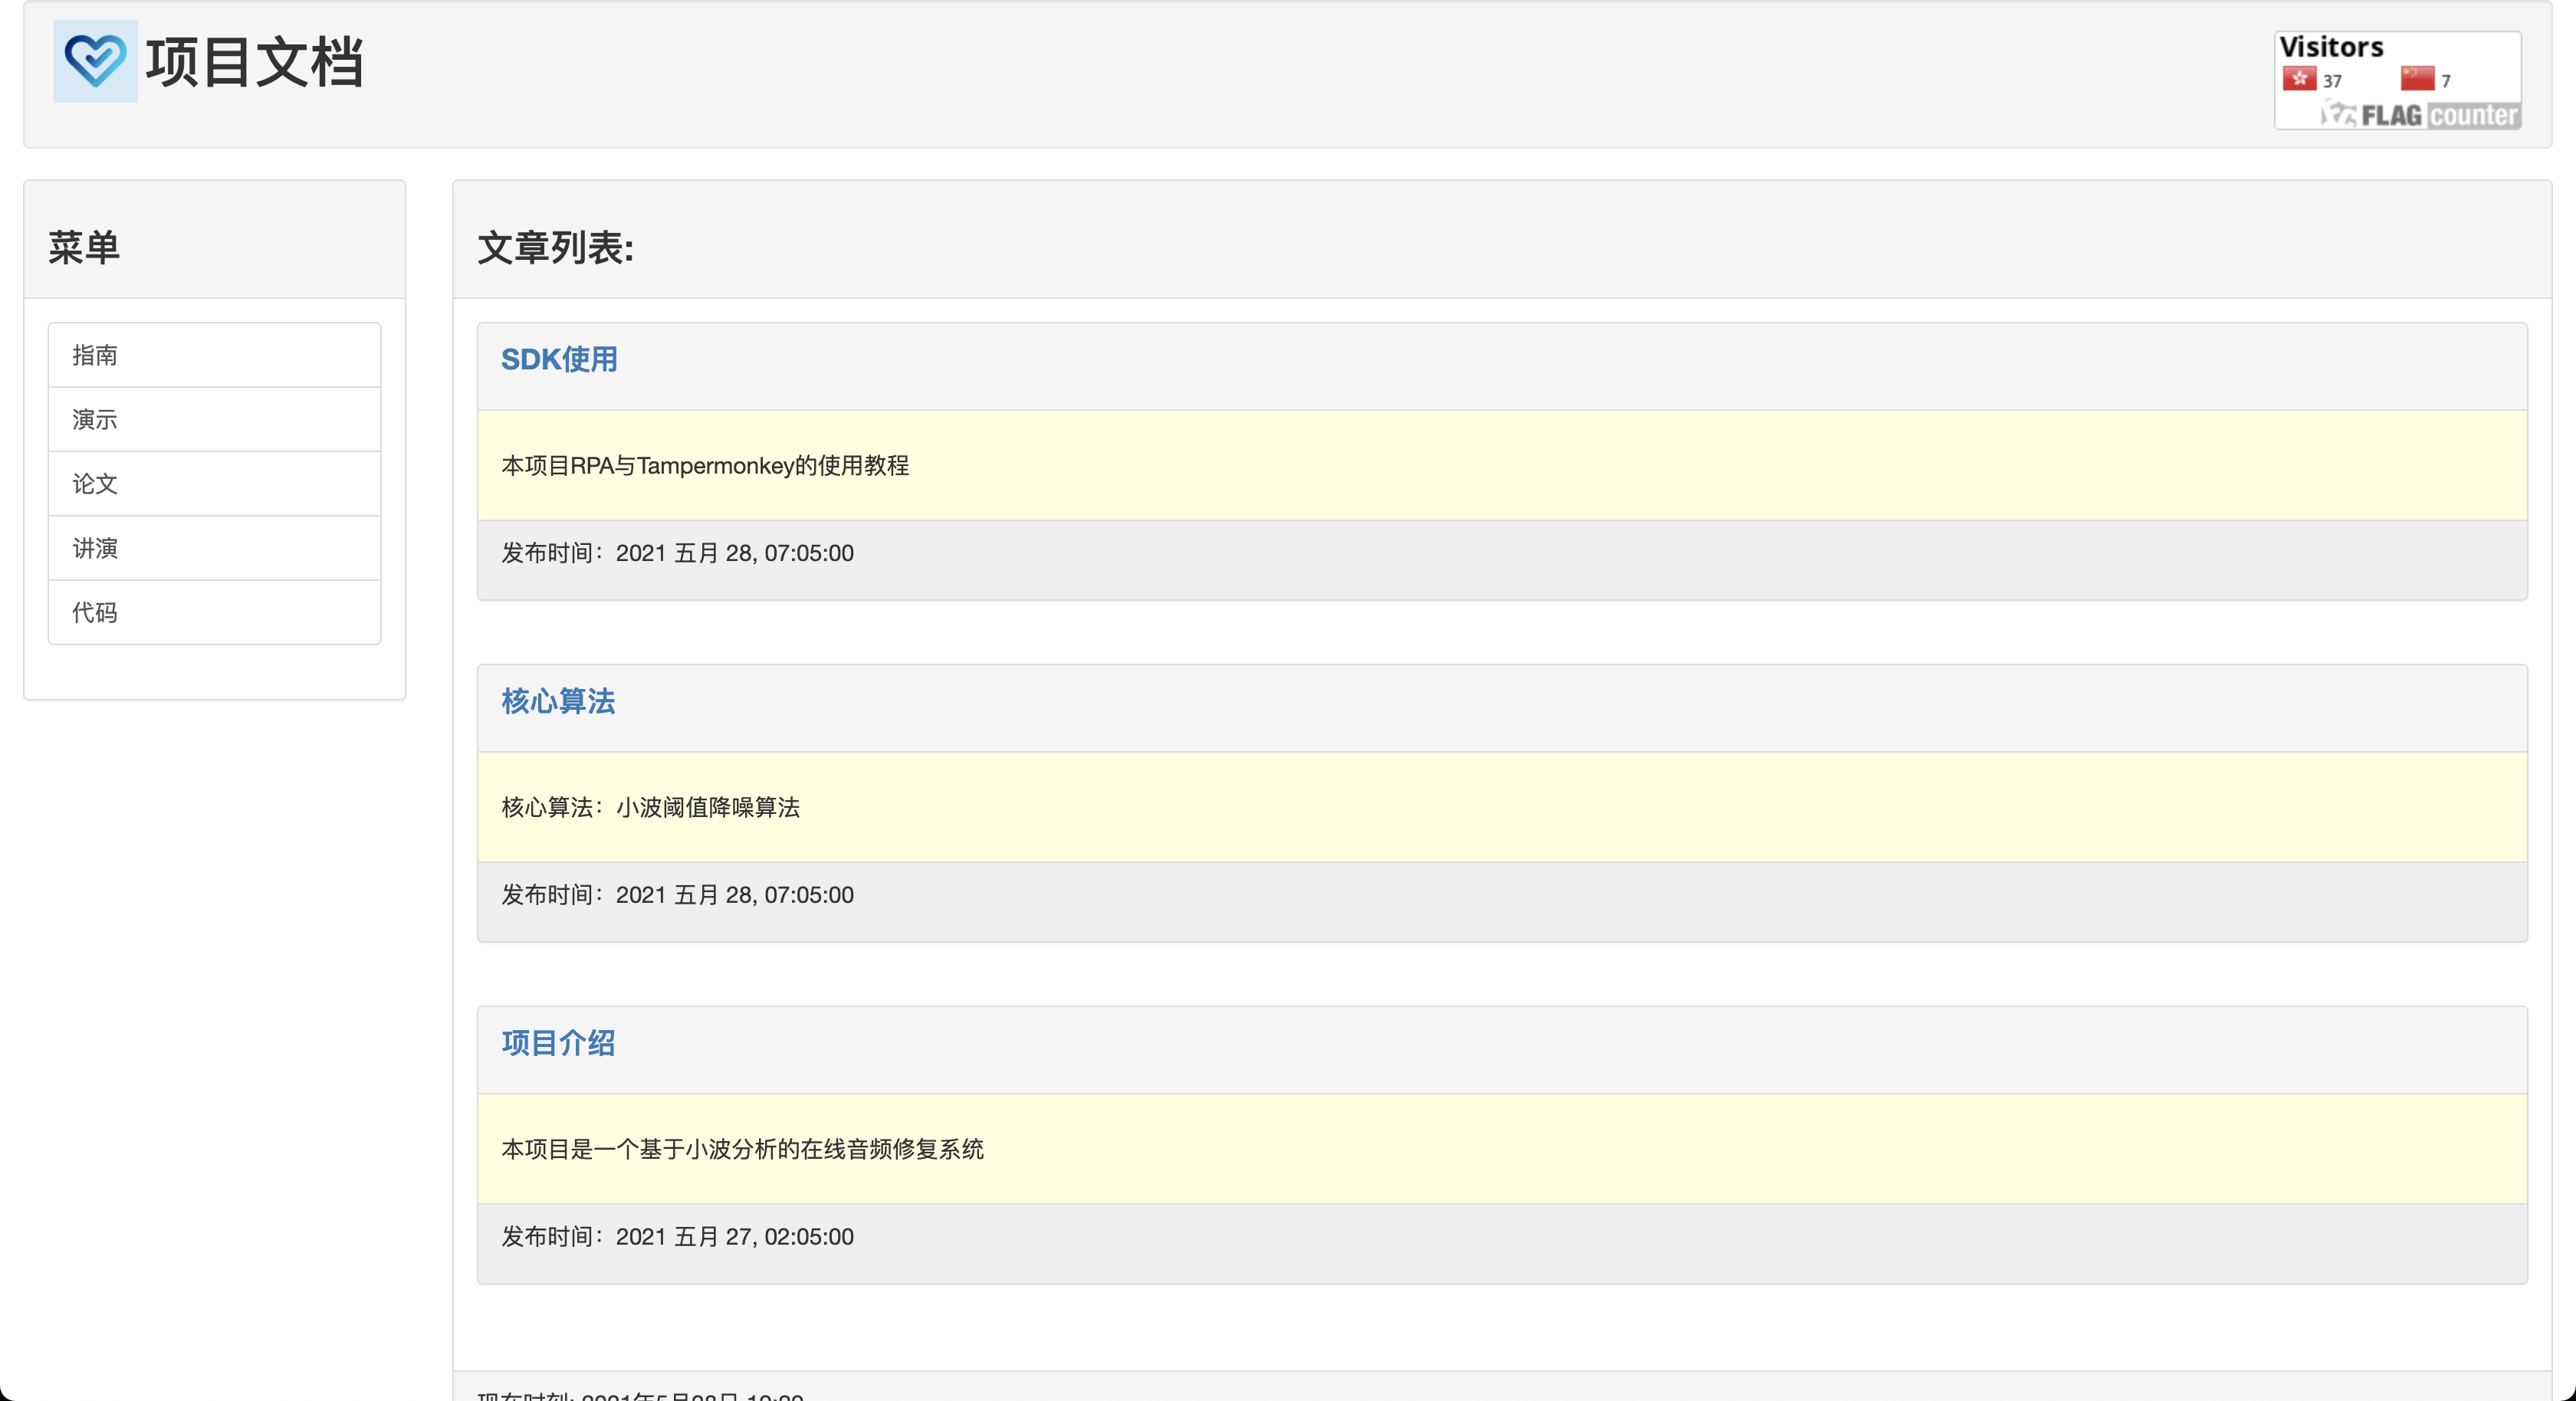
\includegraphics[width=0.7\textwidth]{image/section4/doc.png}
    \captionWithStar{项目文档界面}
\end{figure}

主界面上只显示页面标题、访客量、外链菜单、文章标题及摘要；
点击文章标题后就可以跳转到正文部分。


\paragraph{后端实现}
此模块的文章更新不同于Hugo、Jekyll这一类静态博客，直接使用后台数据库做文章更新；
为了排版便捷，使用markdown2这一类Django插件支持markdown写作。

\subsubsection{高效运行与云端交付}

\paragraph{高效运行}

在开发中，不必过多强调运行效率，而是应该强调需求的快速满足；
但在实际部署中，项目的运行效率就显得尤为重要。

考虑到本项目是在由Python驱动的Django框架下开发的，而Django本身框架下只使用一个线程对请求做出处理。
因为这一设计，导致一旦遇到阻塞IO(Blocking IO,BIO)，Django框架下的view无法处理新的请求。 

此外，由于Python中全局解释锁(Global Interpreter Lock,GIL)的存在，每个线程只有拿到GIL后才能运行，
这就使得python的单核多线程表现很差，只适合应对IO密集型任务；
对于多核多线程而言则更糟，因为CPU0刚释放GIL，其它CPU被唤醒并参与竞争时，GIL有大概率被CPU0抢到，其他的CPU只能再次进入带调度状态，使得效率更低。
这显然不适合本平台的CPU密集型任务需求。

根据上文的分析，结论是只有使用框架外的工具才能实现高效运行。
本项目采用Django+Nginx+Gunicorn的方式来实现高并发，具体方法如图\ref{高效运行}: 

\begin{figure}[htbp]
    \centering
    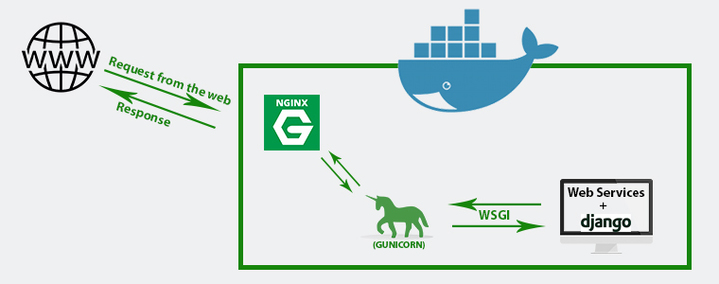
\includegraphics[width=0.7\textwidth]{image/section4/高效运行.png}
    \captionWithStar{高效运行}
\end{figure}


\begin{enumerate}
\item \emph{静态文件}: 考虑到Django响应大量静态文件访问请求时会严重影响性能，
所以让Django在运行时收集所有的静态文件到static文件夹，让高并发的Nginx作为静态服务器响应这些请求。
\item \emph{动态请求}: 使用Gunicorn的CPU模拟器功能来实现多核多进程，实现更好的动态请求响应。
\end{enumerate}


\paragraph{云端交付}
由于本项目涉及的依赖众多，即便使用pipenv同步虚拟环境，但测试系统本身的依赖仍需要妥善解决，这导致了迁移成本较高。

本项目选用Linux容器(Docker)作为迁移工具，它虚拟化操作系统，提供一个额外的软件抽象层
将应用程序及其依赖打包到一个文件中，
允许用户过简单易用的接口，就能让应用程序布署在软件容器下的工作可以自动化进行，大大提高软件交付的速度。\cite{docker1}

本项目生成的镜像如图\ref{docker镜像}所示: 

\begin{figure}[htb]
    \centering
    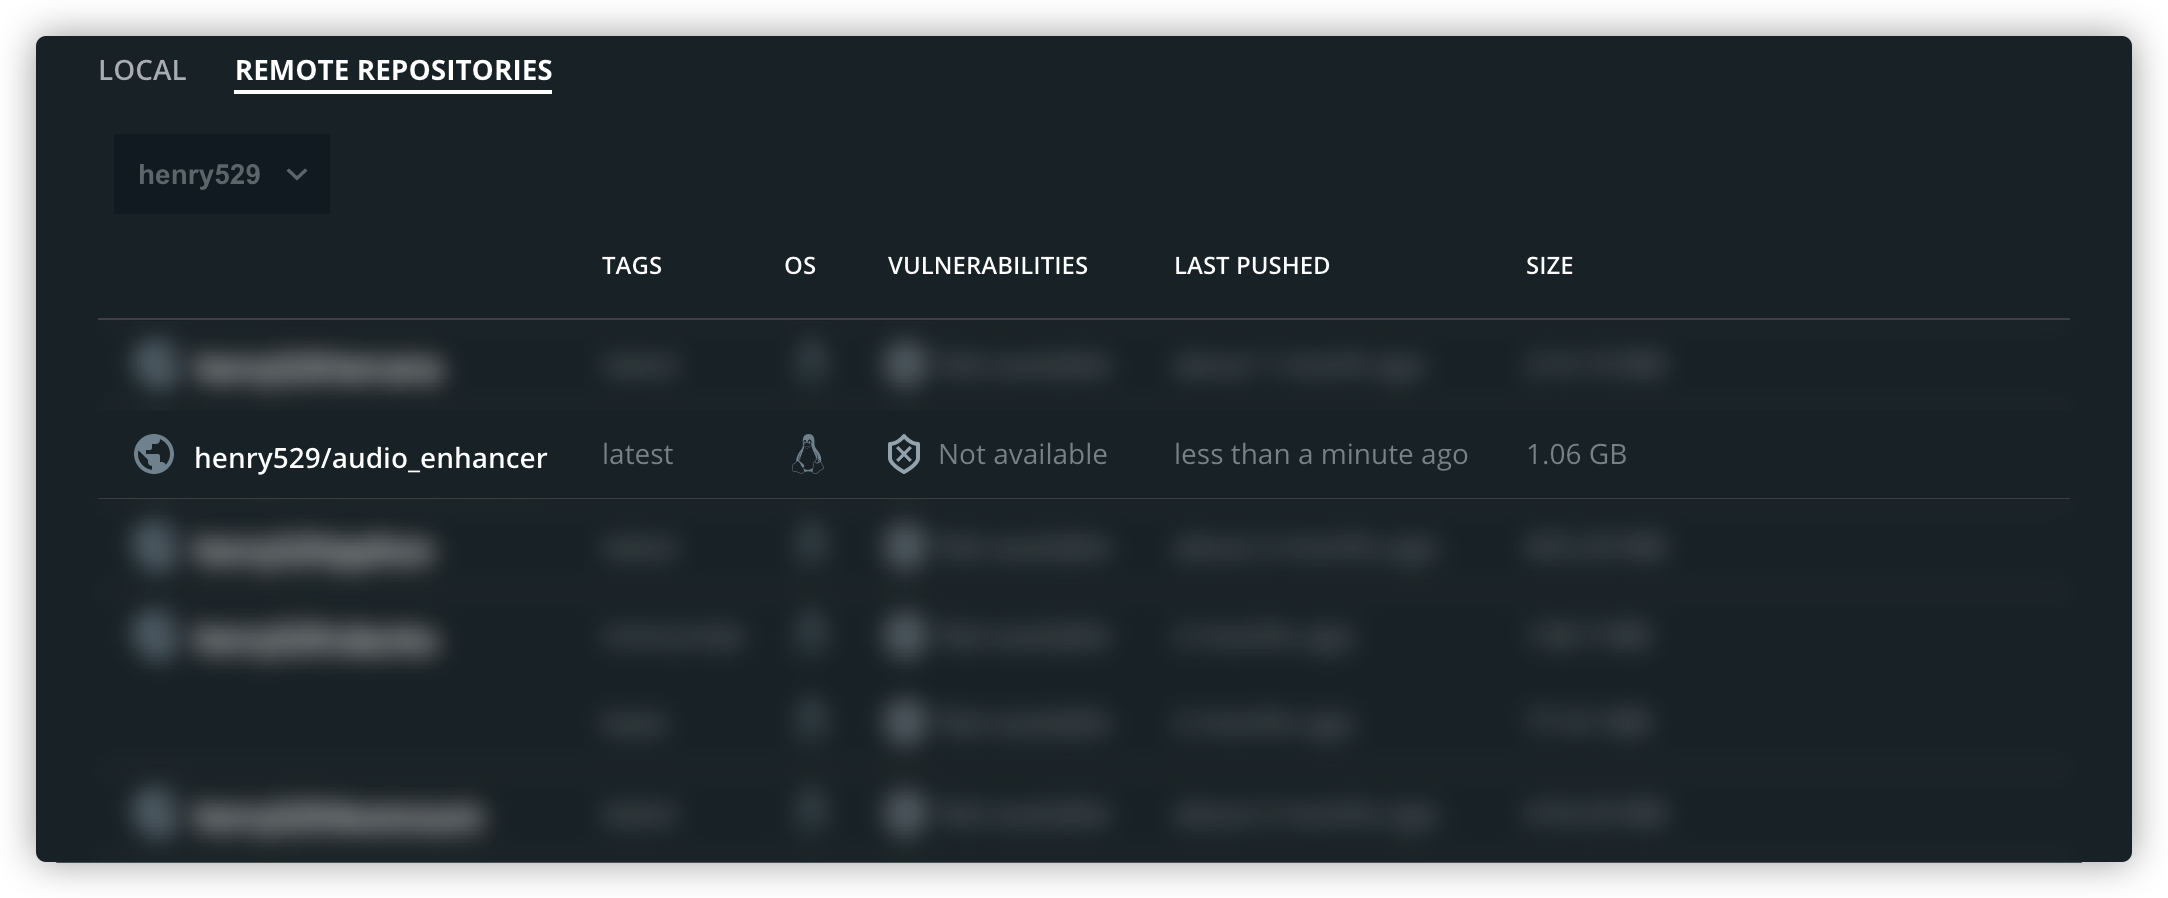
\includegraphics[width=0.75\textwidth]{image/section4/docker-image.png}
    \captionWithStar{docker镜像}
\end{figure}

如图\ref{docker部署流程}所示，生成的镜像通过docker push [image\_name]可以推送到Dockerhub这一类的registry, 
想要复原整个环境只要docker pull [image\_name]就能实现。

\begin{figure}[htb]
    \centering
    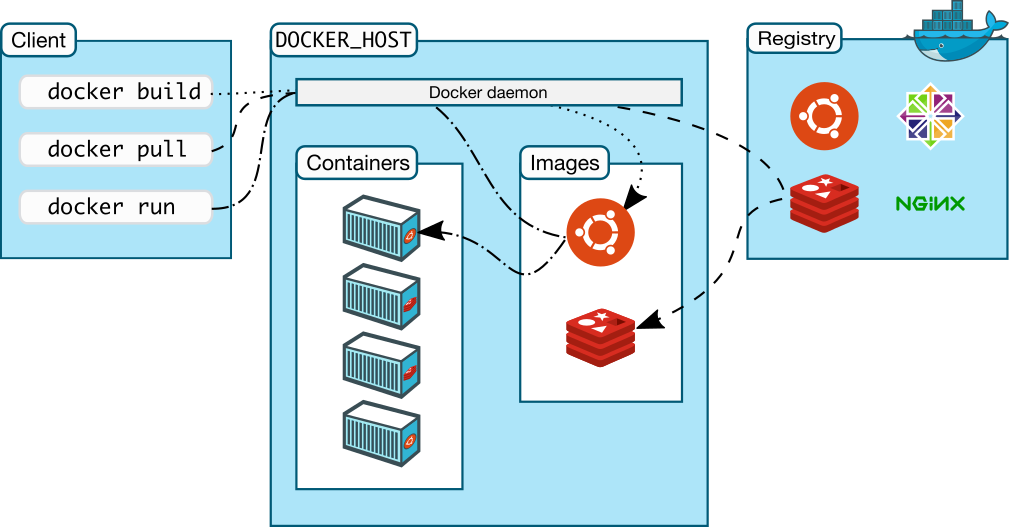
\includegraphics[width=0.75\textwidth]{image/section4/docker-workflow.png}
    \captionWithStar{docker部署流程}
\end{figure}


\subsubsection{Web自动化测试}

机器人流程自动化(Robotic Process Automation, RPA)
是一类能够在当前业务系统结构不变的前提下，实现业务流程自动化的软件工具。\cite{rpa1}
\begin{figure}[htbp]
    \centering
    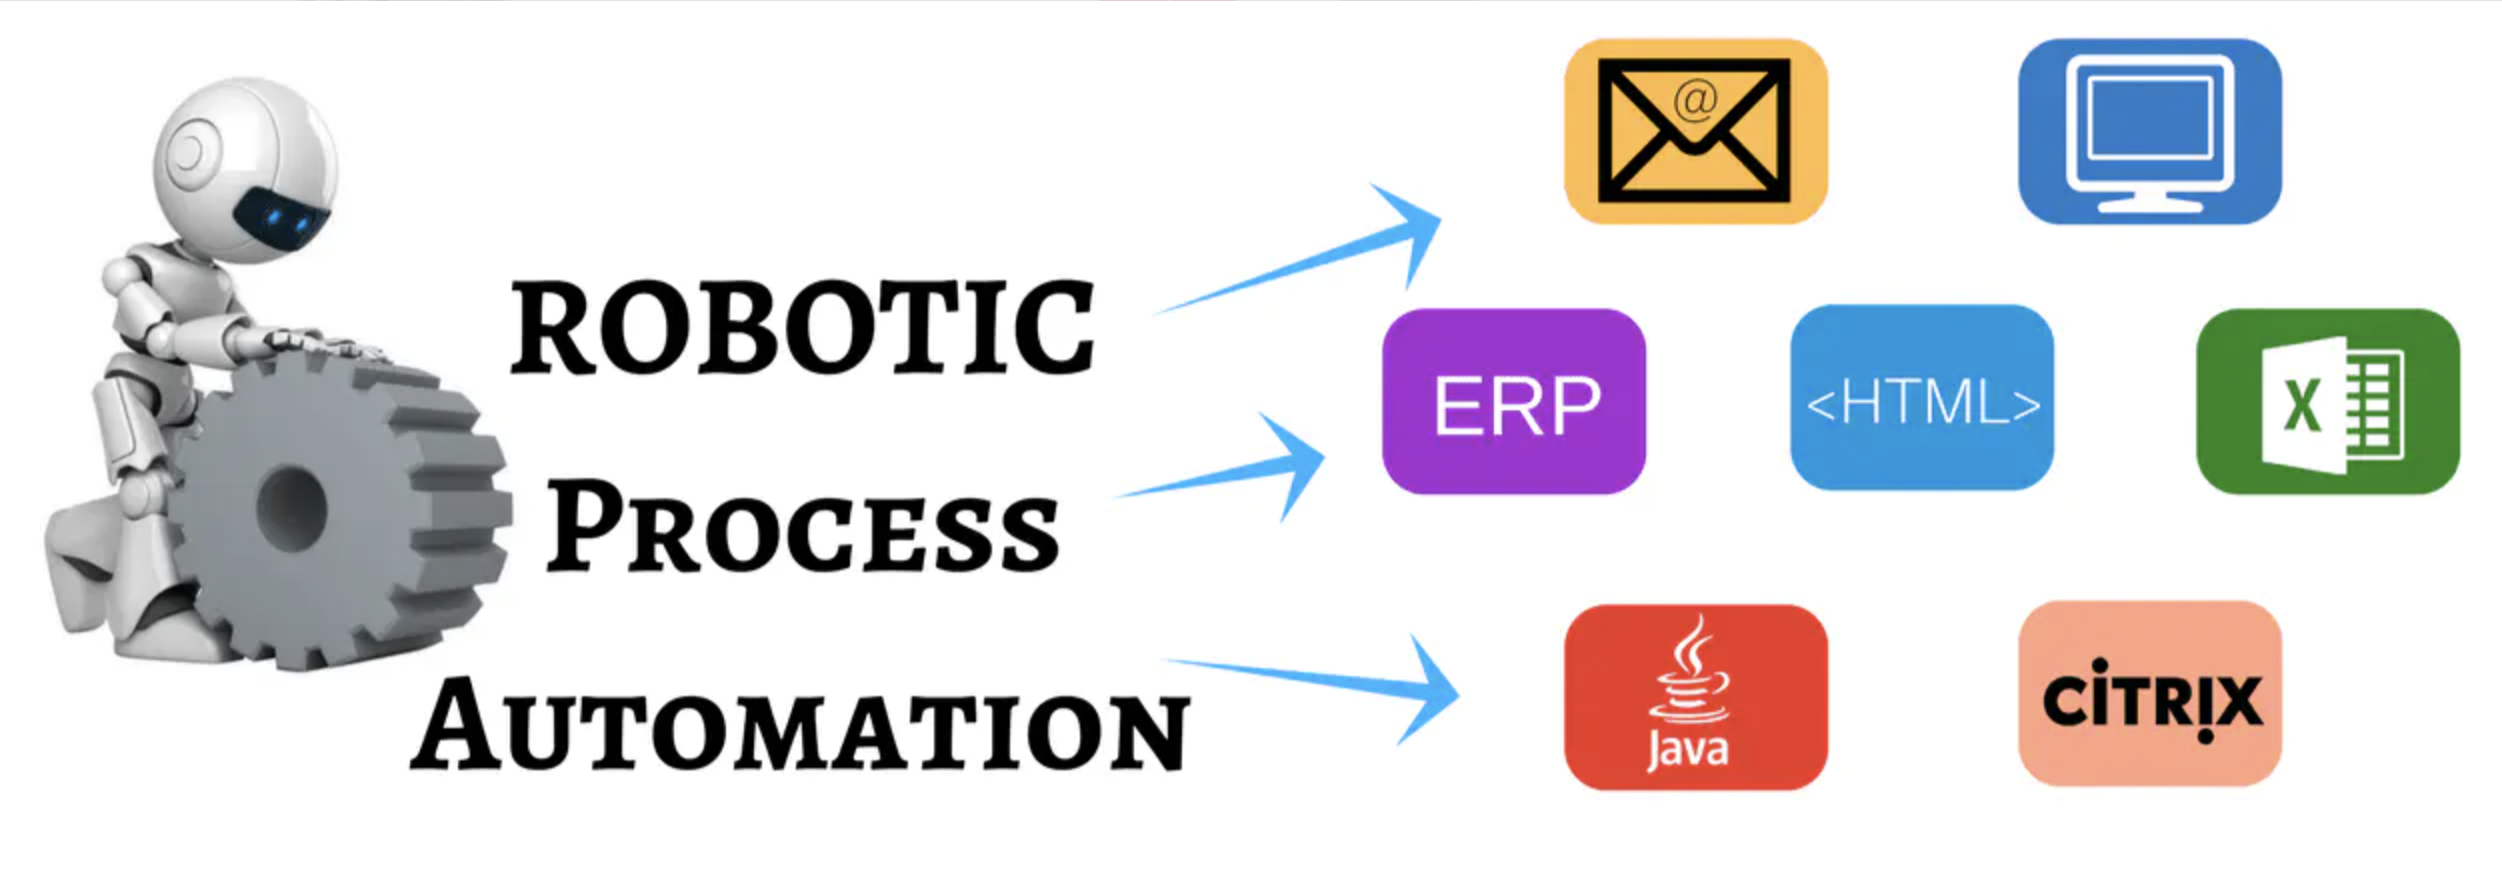
\includegraphics[width=0.8\textwidth]{image/section4/rpa.png}
    \captionWithStar{测试流程自动化}
\end{figure}
为了辅助二次开发，本项目通过Selenium库设计并实现了Web自动化测试工具，用来高效率的完成应用测试。
目前套件中已经封装了如下功能:
\begin{enumerate}
\item 适配主流浏览器的WebDriver；
\item 伪装访问请求；
\item 登录与破解人机验证；
\item 定位页面重要元素；
\item 使用无头浏览器进行全流程测试；
\item 保存重要数据，生成日志。
\end{enumerate}

举例来说: 
在进行登录界面测试时，因为表单中调用了Google Recaptcha来做人机验证，
要想进行下一步就必须通过复杂的图片或音频识别，这在测试中很不方便。
因此本项目提供了是用了SpeechRecognition将获取到的音频转化为文字，并通过selenium将文字输入测试文本框，
实现自动化的登录。








\subsection{本章小结}
本章描述了项目所依托的在线展示平台从需求分析到概要设计，再到具体实现的全过程。
\begin{enumerate}
\item \emph{需求分析}: 具体包括可行性分析(经济可行性、技术可行性)、功能性需求分析(模块需求)和非功能性需求分析(安全性、易用性、可扩展性和可维护性)。
\item \emph{概要设计}: 依据需求分析得出的需求点对平台做出概要设计(架构设计、模块划分以及数据库设计)，
最终将平台设计成具有六层架构(硬件抽象层、数据层、后端中间层、应用层、前端中间层、表现层)和五大模块(数据管理模块、登录注册模块、音频修复模块、意见反馈模块、项目文档模块)的复杂在线系统。
\item \emph{具体实现}: 不仅阐述了开发平台的搭建、各模块的具体实现和云端的部署交付技术，还为二次开发提供了非常便捷的RPA测试工具。
\end{enumerate}




\clearpage
\section{系统测试}

完成项目部署后，在上线前还需要对项目进行一系列测试，包含各模块的功能测试
、对主要操作系统和浏览器的兼容性测试以及关于网站性能的压力测试。

\subsection{功能测试}

在MacOS上的Chrome浏览器，测试如下指标: 

\begin{enumerate}
\item \emph{数据管理模块}: 超级用户的登录与注销、用户与用户组管理、音频数据；
\item \emph{登录注册模块}: 普通用户的登录、访客的内测申请与许可；
\item \emph{音频修复模块}: 音频选择、音频上传、音频修复、音频下载；
\item \emph{意见反馈模块}: 分别测试主题包含“注册”、“问题”以及其它的邮件发送和处理；
\item \emph{项目文档模块}: 项目文档的查看、访问检测；
\end{enumerate}

\begin{table}[htbp]
    \centering
    \captionWithStar{功能测试}
    \begin{tabular}{p{2cm}p{11cm}p{1cm}}
    \thickhline
    \textbf{模块}       & \textbf{功能点} & \textbf{结果}  \\ 
    \thickhline
    \textbf{数据管理}  &  超级用户的登录与注销、用户与用户组管理、音频数据 &  通过 \\
    \textbf{登录注册}  &  普通用户的登录、访客的内测申请与许可 &  通过 \\
    \textbf{音频修复}  &  音频选择、音频上传、音频修复、音频下载 &  通过 \\
    \textbf{意见反馈}  &  分别测试主题包含“注册”、“问题”以及其它的邮件发送和处理 &  通过 \\
    \textbf{项目文档}  &  项目文档的查看、访问检测 &  通过 \\
    \thickhline 
    \end{tabular}
\end{table}

\subsection{兼容性测试}
为了确保在线系统全平台可用，需要针对各个操作系统和浏览器进行测试。

\begin{itemize}
\item \emph{操作系统}: MacOS Big Sur 11.4, Windows 10 21H1, Ubuntu 20.04；
\item \emph{浏览器}: Chrome 90.0, Edge 91.0, Yandex 21.5, Vivaldi 3.8, Opera 76.0, Safari 14.1, Firefox 88.0； 
\item \emph{测试内容}: 页面能否访问、页面响应是否合理以及各模块功能是否可以实现；
\end{itemize}

结果如表\ref{兼容性测试结果}:

\begin{table}[htbp]
    \centering
    \captionWithStar{兼容性测试结果}
    \begin{tabular}{|p{3.3cm}|p{1.2cm}<{\centering}|p{1.2cm}<{\centering}|p{1.2cm}<{\centering}|p{1.2cm}<{\centering}|p{1.2cm}<{\centering}|p{1.2cm}<{\centering}|p{1.2cm}<{\centering}|}
    \hline
    \diagbox{\textbf{操作系统}}{\textbf{测试结果}}{\textbf{浏览器}}  & \textit{Chrome} & \textit{Edge} & \textit{Yandex} & \textit{Opera} & \textit{Vivaldi}  & \textit{Safari} & \textit{Firefox} \\ 
    \hline
    \textbf{MacOS}    & 通过 & 通过 & 通过 & 通过 & 通过 & 通过 & 通过 \\ 
    \hline 
    \textbf{Windows}  & 通过 & 通过 & 通过 & 通过 & 通过 & /   & 通过 \\ 
    \hline
    \textbf{Ubuntu}   & 通过 & /   & 通过 & 未通过 & 未通过 & /   & 通过 \\ 
    \hline
    \end{tabular}
\end{table}

\subsection{压力测试}

网站上线前，还需要做一个压力测试。
使用开源工具Siege在保持每个并发连接次数不变的情况下，无延迟的随机测试网站上5个常见url: 
\begin{enumerate}
\item http://audio.morningstar529.com/
\item http://audio.morningstar529.com/doc/
\item http://audio.morningstar529.com/paper/
\item http://audio.morningstar529.com/slide/
\item http://audio.morningstar529.com/media/images/before.png
\end{enumerate}
结果如下表所示:

\begin{table}[htbp]
    \centering
    \captionWithStar{压力测试}
    \begin{tabular}{lrrrrrrr}
    \thickhline
    Concurrent                           & \textbf{100} & \textbf{200} & \textbf{300} & \textbf{400} & \textbf{500} & \textbf{600} & \textbf{700} \\
    \thickhline
    \textbf{Transactions}(hits)          & 1500         & 2997         & 4485         & 5916         & 7101         & 8223         & 8175         \\
    \textbf{Availability}(\%)            & 100.00       & 99.97        & 99.89        & 99.53        & 98.16        & 96.95        & 91.34        \\
    \textbf{Elapsed time}(secs)          & 29.14        & 58.68        & 128.38       & 214.66       & 225.92       & 266.41       & 313.78       \\
    \textbf{Data transferred}(MB)        & 216.01       & 431.60       & 645.88       & 214.66       & 1022.61      & 1184.19      & 1177.28      \\
    \textbf{Response time}(secs)         & 1.64         & 2.98         & 4.49         & 5.92         & 7.42         & 15.19        & 15.75        \\
    \textbf{Transaction rate}(trans/sec) & 51.48        & 51.07        & 34.94        & 27.56        & 31.43        & 30.87        & 26.05        \\
    \textbf{Throughput}(MB/sec)          & 7.41         & 7.36         & 5.03         & 3.97         & 4.53         & 4.44         & 3.75         \\
    \textbf{Concurrency}                 & 84.23        & 152.16       & 156.83       & 163.14       & 233.15       & 468.80       & 410.43       \\
    \textbf{Successful transactions}     & 1500         & 2997         & 4486         & 5916         & 7101         & 8229         & 8176         \\
    \textbf{Failed transactions}         & 0            & 1            & 5            & 28           & 133          & 259          & 775          \\
    \textbf{Longest transaction}         & 9.01         & 18.26        & 46.62        & 49.82        & 42.72        & 91.03        & 57.39        \\
    \textbf{Shortest transaction}        & 0.13         & 0.13         & 0.12         & 0.22         & 0.14         & 0.14         & 0.13         \\
    \thickhline
    \end{tabular}
\end{table}

\subsection{本章小结}
本章节罗列了各个模块的功能测试，包括数据管理模块、登录注册模块、音频修复模块等，功能点全部顺利实现；

为了保证该在线系统全平台兼容，本章在主流的操作系统与浏览器上都进行了在线系统的音频修复全流程测试，除去浏览器本身不稳定的因素，
本系统兼容性与预期一致，足以满足用户多样化的需求；

此外，还对在线系统做了压力测试，整个过程中在线系统并无不良反应，运行稳定，并发能力在当前阶段足以满足需求。


\clearpage
\sectionWithStar{总结和展望}

本文主要包含两个方面：基于小波软硬折中阈值的小波阈值去噪算法的研究与基于Django的在线音频修复平台设计。

虽然在小波降噪领域与网络应用开发方面都做出了一定成果，但由于时间精力有限，
现阶段仍然有很多不足：
\begin{enumerate}
\item 新的软硬折中阈值算法没有从根本上解决阈值附近不连续以及阈值以上小波系数被压缩的问题。
\item 降噪过程中，没有考虑到清音的高频特性，造成了语音信号的损失。 
\item 脉冲噪声噪点获取过程中未充分发挥矩阵运算的效率，降低了算法的效率。
\item 本项目使用的Django框架由于原生单线程以及GIL的存在，并发效率低。
\end{enumerate}

后续工作可以按照下面的思路开展：
\begin{enumerate}
\item 找寻一个既连续又能较好的保持阈值以上小波系数不变的阈值函数。
\item 结合语音中清浊音的特点处理信号，减少有用信号的损失。
\item 修复算法实现过程中要充分发挥矩阵运算的效率，减小算法的时间复杂度。
\item 替换当前的Django框架，提高网站的综合性能。
\end{enumerate}


\clearpage

\addbib{paper.bib}



\clearpage
\sectionWithStar{致谢}
大学四年时光匆匆而过，我首先感谢母校，在这四年里给我提供了一个良好的生活环境和学习环境，让我在这四年大学生活中学有所成。

其次，我要感谢我的毕设导师李义丰老师，他在论文撰写方面给我提了很多重要的方法和意见，在此，向李老师致以由衷的感谢和敬意。

我还要感谢我的父母，他们不辞劳苦供我读书，一直以来默默的为我付出，是我最坚实的后盾，真心地感谢他们的关爱。

最后还要感谢谷歌公司为本次的毕设工作提供了免费服务器与技术支持的，创造了在线修复的可能性。

\begin{comment}
作为一家商业公司，你们不作恶以及开放包容的理念真的是打动人心的。
最后还要感谢被薅了多次羊毛的谷歌公司，不仅免费用了你们两年的服务器，还在本项目中同时使用了你们的语音认证与语音识别API(最后证明矛还是比盾坚硬)，
作为一家商业公司，你们不作恶以及开放包容的理念真的是打动人心的。
\end{comment}

大学四年生活虽然落下帷幕，但人生却远不会止步于此。
未来的日子也许充满荆棘，也许一切顺遂，怀着对生活的憧憬、对未来的敬畏，过好每一天，希望毕业顺利的同时，一切如意！


\begin{comment}
\startappendix
\section{正交小波推导}
\clearpage
\section{Daubechies小波推导}
\end{comment}

\end{document}




